% !TeX root = ../../Book3.tex
% 纲要标题：## 第11章　Sobolev 空间、紧性与几何不等式
% 纲要位置：几何学计划纲要.md，第 2501 行。
% 正文状态：初稿；尚未正式审核。

% 纲要内容开始
% 
% > 本章目标与证明范围：必要的泛函分析和流形上的局部化在本章系统建立。嵌入的指数、丛值版本和几何常数分别说明，为后续估计提供真正可使用的工具。
% 
% 纲要内容结束

\chapter{Sobolev 空间、紧性与几何不等式}
\label{g3:ch:11}
\BookChapterNumber{g3:ch:11}

\begin{chapterabstract}
控制一个函数及其导数的积分，能够得到怎样的连续性、紧性与边界值？本章先用体积密度定义丛值积分，从测试截面、分布与弱协变导数构造整数阶 Sobolev 空间，证明完备性、光滑稠密性、乘法与链式法则，并建立弱紧性所需的泛函分析。随后由 Euclid 积分估计推出 Sobolev 与 Morrey 嵌入，逐项辨清临界指数；通过连通覆盖证明 Poincaré 不等式，通过平移控制与有限近似证明 Rellich 紧性。最后在边界图中构造延拓、定义迹并刻画零边界空间，为下一章的弱椭圆方程准备函数空间与估计。
\end{chapterabstract}

\begin{learninggoals}
\begin{itemize}
	\item 从测试配对识别弱导数，说明密度、局部标架和联络在丛值公式中的作用。
	\item 构造整数阶 Sobolev 空间，掌握光滑逼近、乘法、复合与截断的适用条件。
	\item 区分强收敛与弱收敛，并由反射性和可分对偶提取弱收敛子列。
	\item 计算嵌入指数及缩放，辨别临界端点、连续代表与高阶乘法估计。
	\item 用零边界或零均值条件消除常数核，追踪覆盖与几何退化对估计常数的影响。
	\item 证明紧嵌入与迹估计，识别零迹、补零延拓和零边界闭包之间的关系。
\end{itemize}
\end{learninggoals}

在区间上，函数 \(u(x)=|x|\) 在原点不可微，但它的斜率在两侧都有界，能量 \(\int|u'|^2\) 仍有自然意义。若用光滑函数逼近这个尖点，函数和一阶导数都可以在积分范数中收敛。一个容纳能量极限的函数空间，应当保留这样的函数，并把导数解释为分部积分中的对象。Sobolev 空间\footnote{Sergei L'vovich Sobolev（1908—1989），苏联数学家，研究偏微分方程、广义函数与泛函分析；以弱导数和积分范数研究函数正则性的空间以其命名。}由此把经典微分运算延伸到较大的完备空间。

\ProseParagraphBreak

范数有界与收敛仍是两件事。在圆周上，\(u_j(x)=j^{-1}\sin(jx)\) 一致趋零，导数 \(\cos(jx)\) 的平方积分却保持不变。它们的导数只能在测试配对意义下趋零。另一方面，把同一个小凸起搬到越来越远的位置，会使所有局部观察都趋零，却保留全局范数。本章分别用弱紧性与强紧性处理这些现象：前者保留线性配对和能量下界，后者需要控制振荡、集中与质量远移。

\ProseParagraphBreak

嵌入定理给出导数控制所能换取的积分指数或连续性。指数由缩放决定，边界条件与连通性则决定能否只用导数控制函数本身。把 Euclid 估计移到流形上，还须写清坐标、度量、联络及截断函数带来的常数。上一章的塌缩例子提醒我们：每个固定流形上的估计成立，并不自动给出一个变化几何族上的统一常数。

\ProseParagraphBreak

本章使用第一章的体积密度、联络与散度，以及坐标图、单位分解和基本测度与积分。积分换序、收敛定理、Euclid 测度的内外正则性，以及有限有符号测度对有限正测度绝对连续时的积分密度表示，作为实分析基础使用；弱导数、函数空间和所需泛函分析则在这里建立。为避免将边界问题隐入记号，闭流形、有界延拓域与零边界空间的结论分别陈述。对照阅读可查 Brezis 的第4.3节关于 \(L^p\) 对偶与反射性的讨论，以及第9.1—9.4节关于弱导数、延拓、嵌入与零边界空间的内容\cite[第4.3节，第9.1—9.4节]{Brezis2011}。

% !TeX root = ../../Book3.tex
% 纲要标题：### 11.1 积分、分布和弱微分
% 纲要位置：几何学计划纲要.md，第 2505 行。
% 正文状态：初稿；尚未正式审核。

% 纲要内容开始
% 
% * 体积密度及 Lᵖ 截面
% * 测试截面和分布
% * 弱导数与分部积分
% * 局部平凡化和坐标变换
% 
% 纲要内容结束

\section{积分、分布和弱微分}
\label{g3:sec:1101}

一列光滑函数可以有收敛的能量，而极限在个别点没有经典导数。例如 \(u_\varepsilon(x)=\sqrt{x^2+\varepsilon^2}\) 在有界区间上趋向 \(|x|\)，其一阶导数有一致界。若把导数移到紧支测试函数上，极限仍满足同一个积分恒等式。弱微分正是用这种稳定的恒等式记录导数；在向量丛上，还要让测试对象与换标架相容。

\subsection{\texorpdfstring{体积密度及 \(L^p\) 截面}{体积密度及 Lᵖ 截面}}
\label{g3:subsec:1101:01}
第一章的体积密度\cref{g3:def:metric-volume-density}在坐标中为 \(\mu_g=m(x)|\mathrm dx|\)，其中 \(m=\sqrt{\det(g_{ij})}>0\)。对非负可测函数，取局部有限单位分解 \(\{\chi_a\}\)，定义
\[
	\int_M f\,\mu_g=\sum_a\int_{x_a(U_a)}(\chi_af)\circ x_a^{-1}\,m_a\,\mathrm dx.
\]
这里右边采用 Lebesgue 积分。\footnote{Henri Léon Lebesgue（1875--1941），法国数学家，建立了现代测度与积分理论，并研究实变函数与三角级数。}在两套分解之间插入 \(\sum_b\widetilde\chi_b=1\)，再用非负积分的求和交换和坐标换元，得到相同数值。对可积的有符号函数按正负部分定义。这个构造不要求定向；第二可数性使流形可由可数个相对紧坐标片覆盖，因而所得测度是 \(\sigma\)-有限的。

\begin{definition}\label{g3:def:lp-sections}
	设 \((M,g)\) 为光滑黎曼流形，\(E\to M\) 为有限秩实或复光滑向量丛，配有光滑正定纤维度量 \(h\)。若截面的局部分量可测，就称截面可测。将几乎处处相等的截面识别，定义
	\[
		\|s\|_{L^p(E)}=\left(\int_M|s|_h^p\,\mu_g\right)^{1/p}
		\quad(1\le p<\infty),\qquad
		\|s\|_{L^\infty(E)}=\mathop{\mathrm{ess\,sup}}_M|s|_h.
	\]
	范数有限的空间记为 \(L^p(M;E)\)；在每个相对紧坐标片上可积的版本记为 \(L^p_{\mathrm{loc}}(M;E)\)。平凡线丛时省略 \(E\)。
\end{definition}
\symidx{\(L^p(M;E)\)：有限秩向量丛的可积截面空间}

光滑可逆过渡矩阵保持可测性，并在紧集上连同其逆一致有界。因此上述可测性与局部可积性不依赖标架。\(L^p\) 的元素是等价类：单个点上的取值一般尚无定义。

\begin{proposition}\label{g3:prop:lp-basic}
	设 \(E\to(M,g)\) 为上述有限秩度量丛，\(1\le p\le\infty\)，\(1/p+1/p'=1\)。则 \(L^p(M;E)\) 是完备赋范空间。对 \(s\in L^p(E)\)、\(\eta\in L^{p'}(E^*)\)，有
	\[
		\int_M|\eta(s)|\,\mu_g\le\|\eta\|_{p'}\|s\|_p.
	\]
	若 \(A\subset M\) 可测、\(0<\mu_g(A)<\infty\)，且 \(1\le q\le p\le\infty\)，则
	\[
		\|s\|_{L^q(A)}\le\mu_g(A)^{1/q-1/p}\|s\|_{L^p(A)}.
	\]
\end{proposition}
\begin{proof}
	当 \(1<p<\infty\) 时，凸函数的切线不等式给出 \(ab\le a^p/p+b^{p'}/p'\)。先把两个函数各除以自己的范数，再积分，便得 Hölder 不等式；端点由本质上界直接得到。最后一个结论是将它用于 \(|s|^q\) 与常数一。三角不等式在 \(p=1,\infty\) 时直接成立；其余情形将 \(|s+t|^{p-1}\) 与 \(|s|+|t|\) 配对，得到 \(\|s+t\|_p^p\le(\|s\|_p+\|t\|_p)\|s+t\|_p^{p-1}\)，再除去公共因子。\footnote{Otto Ludwig Hölder（1859--1937），德国数学家，研究分析中的不等式与连续性，也对群论作出重要贡献。}

	证明完备性时，先从任意 Cauchy 列选出子列，使相邻差的范数不超过 \(2^{-j}\)。当 \(p<\infty\) 时，部分和 \(\sum_{j\le N}|s_{j+1}-s_j|\) 的 \(L^p\) 范数至多为一；单调收敛说明其极限几乎处处有限。故在这些点上，纤维中的向量级数绝对收敛，得到可测截面 \(s\)。余项的 \(L^p\) 范数至多为 \(\sum_{j\ge N}2^{-j}\)，所以子列强收敛；原列的 Cauchy 性给出整列强收敛。\(p=\infty\) 时去掉可数个零测集后，各相邻差都满足同一逐点上界，故级数一致收敛，结论相同。
\end{proof}

完备赋范空间称为\term[Banach kongjian]{Banach 空间}[Banach space]。\footnote{Stefan Banach（1892--1945），波兰数学家，奠定现代泛函分析的重要基础，研究赋范空间、线性算子及积分。}完备性保证范数意义下的近似不会跑出所选空间。有限测度上的最后一个估计还表明，提高可积指数会加强控制，但其常数带有体积因子。

\begin{lemma}\label{g3:lem:lp-smooth-density}
	在 \(\mathbb R^n\) 的开集 \(\Omega\) 上，\(C_c^\infty(\Omega)\) 在 \(L^p(\Omega)\) 中稠密，\(1\le p<\infty\)。同样的结论对光滑流形上的有限秩度量丛成立。
\end{lemma}
\begin{proof}
	先截去函数的大值和固定紧集外的部分，误差由可积性趋零；再把有界函数的值域分成小区间，得到有限线性组合的示性函数。前一步所得的可测集 \(A\) 都含于 \(\Omega\) 的固定紧集。测度的内外正则性给出紧集 \(K\) 与相对紧开集 \(V\)，使 \(K\subset A\subset V\Subset\Omega\)，且 \(|V\setminus K|\) 任意小。取光滑函数 \(0\le\chi\le1\)，在 \(K\) 上为一、支集紧含于 \(V\)；这样的函数可用有限个球上的光滑鼓包函数相加，再作光滑截断构造。于是 \(\|\chi-\mathbf1_A\|_p^p\le|V\setminus K|\)。依次逼近简单函数的有限项，便得结论。流形上先用可数相对紧坐标片截取有限部分，再逐分量使用上述论证；紧集上的正密度和纤维范数与 Euclid 版本一致等价。
\end{proof}

\subsection{测试截面和分布}
\label{g3:subsec:1101:02}
弱方程要和足够丰富的测试对象配对。若待求对象是 \(E\) 的截面，自然的测试对象是对偶丛 \(E^*\) 的截面再乘一个密度；这样两者配对后可以直接积分。记密度线丛为 \(|\Lambda|^n\mathrm T^*M\)。

\begin{definition}\label{g3:def:bundle-distribution}
	设 \(E\to M\) 为光滑有限秩向量丛。一个 \(E\) 值\term[fenbu]{分布}[distribution]是测试空间 \(C_c^\infty(M;E^*\otimes|\Lambda|^n\mathrm T^*M)\) 上的线性泛函 \(T\)，满足：对每个紧集 \(K\) 都存在整数 \(m\) 和常数 \(C_K\)，使支集位于 \(K\) 的测试截面 \(\phi\) 满足
	\[
		|T(\phi)|\le C_K\sum_{|\alpha|\le m}\sup_K|\partial^\alpha\phi|.
	\]
	右端用覆盖 \(K\) 的有限个坐标与标架中的分量计算。由有限阶链式法则，该条件不依赖这些选择。分布空间记为 \(\mathcal D'(M;E)\)。
\end{definition}

密度 \(\mu_g\) 固定后，可将测试截面写成 \(\eta\mu_g\)，\(\eta\in C_c^\infty(E^*)\)。对 \(s\in L^1_{\mathrm{loc}}(E)\)，
\[
	T_s(\eta\mu_g)=\int_M\eta(s)\,\mu_g
\]
定义一个分布：紧集上的 \(L^1\) 范数乘测试截面的上界就是连续性估计。对复丛仍用复线性对偶配对；若改用 Hermitian 内积，则约定第一槽线性，测试槽相应取共轭。

\begin{example}\label{g3:exm:point-distribution}
	在 \(\mathbb R\) 的通常密度下，\(\delta_0(\varphi\,|\mathrm dx|)=\varphi(0)\) 是分布。它不是局部可积函数产生的分布：取 \(0\le\varphi_\varepsilon\le1\)、\(\varphi_\varepsilon(0)=1\)、支集在 \((-\varepsilon,\varepsilon)\)，若 \(\delta_0=T_f\)，则 \(1\le\int_{-\varepsilon}^{\varepsilon}|f|\to0\)，矛盾。
\end{example}

分布收敛 \(T_j\to T\) 指对每个固定测试截面都有 \(T_j(\phi)\to T(\phi)\)。局部 \(L^1\) 收敛足以推出这种收敛；分布可以记住集中到一点的质量，因此分布极限未必仍由函数表示。

\subsection{弱导数与分部积分}
\label{g3:subsec:1101:03}
在 Euclid 开集 \(\Omega\) 上，分部积分将经典偏导数写成 \(\int (\partial_i u)\varphi=-\int u\partial_i\varphi\)。右端只要求 \(u\) 局部可积，因而可用它定义弱导数。

\begin{definition}\label{g3:def:weak-derivative}
	设 \(\Omega\subset\mathbb R^n\) 开，\(u,v_i\in L^1_{\mathrm{loc}}(\Omega)\)。若对所有 \(\varphi\in C_c^\infty(\Omega)\) 有
	\[
		\int_\Omega v_i\varphi\,\mathrm dx=-\int_\Omega u\partial_i\varphi\,\mathrm dx,
	\]
	则称 \(v_i\) 为 \(u\) 的第 \(i\) 个\term[ruo daoshu]{弱导数}[weak derivative]，记为 \(\partial_i u\)。一般分布的导数定义为 \((\partial_i T)(\varphi)= -T(\partial_i\varphi)\)，高阶偏导按同一规则迭代。
\end{definition}

这种定义中的导数总作为分布存在；称它为可积弱导数时，额外要求该分布由一个局部可积函数表示。弱导数几乎处处唯一：若局部可积函数 \(f\) 对所有光滑紧支测试函数的积分为零，以紧支连续函数逼近有界可测函数，可得 \(\int_K|f|=0\) 对每个紧集成立，故 \(f=0\) 几乎处处。也可由下面的局部平滑论证直接得到唯一性。

\begin{example}\label{g3:exm:corner-and-jump}
	在 \(\mathbb R\) 上，分别在零点两侧积分，得到
	\[
		\partial_x|x|=\operatorname{sgn}x,\qquad
		\partial_x\operatorname{sgn}x=2\delta_0
	\]
	作为分布恒等式。第一式中的边界贡献因 \(|x|\) 在零点连续而抵消；第二式的两个单侧值相差二，恰留下点质量。折角与跳跃对弱微分产生不同影响。
\end{example}

\begin{lemma}\label{g3:lem:local-weak-smoothing}
	设 \(u\in L^p_{\mathrm{loc}}(\Omega)\)，\(1\le p<\infty\)，且所有 \(|\alpha|\le k\) 的弱导数局部属于 \(L^p\)。取非负光滑函数 \(\rho\)，支集在单位球、积分为一，令 \(\rho_\varepsilon(x)=\varepsilon^{-n}\rho(x/\varepsilon)\)。在距边界大于 \(\varepsilon\) 的点定义 \(u_\varepsilon=\rho_\varepsilon*u\)。则它光滑，且
	\[
		\partial^\alpha u_\varepsilon=\rho_\varepsilon*\partial^\alpha u,
		\qquad \partial^\alpha u_\varepsilon\longrightarrow\partial^\alpha u
		\quad\text{于 }L^p_{\mathrm{loc}}.
	\]
\end{lemma}
\begin{proof}
	核的支集紧含于积分区域，故可将对 \(x\) 的微分移到核上，再按弱导数定义移给 \(u\)，得到交换公式。证明收敛只需零阶情形。先乘一个在所考察紧集附近为一的光滑截断，将问题化到 \(L^p(\mathbb R^n)\)。由\cref{g3:lem:lp-smooth-density}先逼近紧支连续函数；后者的平移在 \(L^p\) 中趋于自身，而平移保持范数，所以一般 \(f\in L^p\) 也满足 \(\|f(\cdot-z)-f\|_p\to0\)。积分三角不等式于是给出
	\[
		\|\rho_\varepsilon*f-f\|_p
		\le\int\rho_\varepsilon(z)\|f(\cdot-z)-f\|_p\,\mathrm dz\longrightarrow0.
	\]
\end{proof}

\begin{proposition}\label{g3:prop:weak-line-slices}
	设 \(Q=I_1\times\cdots\times I_n\) 为有界开矩形，\(u,v_i\in L^1(Q)\)。则 \(\partial_i u=v_i\) 弱成立，当且仅当对几乎每条平行于第 \(i\) 轴的直线，\(u\) 的限制有一个绝对连续代表，且其一元导数等于该直线上的 \(v_i\)。
\end{proposition}
\begin{proof}
	先固定 \(i\)，把其他坐标记为 \(x'\)。弱恒等式用于乘积测试函数 \(\psi(x')\eta(t)\)，交换积分后说明
	\(\int u(x',t)\eta'(t)\,\mathrm dt=-\int v_i(x',t)\eta(t)\,\mathrm dt\)
	对几乎处处 \(x'\) 成立。先对一组在各个紧子区间的 \(C^1\) 范数下稠密的可数测试函数取共同零测例外集，再由积分估计延拓到所有 \(\eta\)。在一维中令 \(V(t)=\int_{t_0}^tv_i(x',\tau)\,\mathrm d\tau\)，则 \(u-V\) 的分布导数为零。任意积分为零的紧支测试函数都是另一个紧支测试函数的导数，因此 \(u-V\) 对测试函数的作用仅依赖其积分；减去一个常数后它为零。这说明 \(u=V+c\) 几乎处处，即有绝对连续代表。反向对每条合格直线作一元分部积分，再交换积分，即得弱恒等式。
\end{proof}

局部 Lipschitz 函数沿这些直线绝对连续，故具有局部本质有界的弱梯度。在 Euclid 坐标中若 Lipschitz 常数为 \(L\)，对可数个稠密单位方向重复上述论证，得到 \(|\mathrm Du|\le L\) 几乎处处。这样取得的是整个梯度的长度界，而不只是各坐标分量分别不超过 \(L\)。

\begin{definition}\label{g3:def:weak-covariant-derivative}
	设 \(E\to(M,g)\) 为光滑有限秩向量丛，配有光滑联络 \(\nabla\)。对 \(s\in L^1_{\mathrm{loc}}(E)\)，若 \(A\in L^1_{\mathrm{loc}}(\mathrm T^*M\otimes E)\) 对所有光滑向量场 \(X\) 及紧支光滑对偶截面 \(\eta\) 满足
	\begin{equation}\label{g3:eq:weak-covariant-parts}
		\int_M\eta(A(X))\,\mu_g
		=-\int_M(\nabla_X^{E^*}\eta)(s)\,\mu_g
		-\int_M\eta(s)\operatorname{div}_gX\,\mu_g,
	\end{equation}
	则称 \(A\) 为 \(s\) 的弱协变导数，记作 \(\nabla s\)。有边界时，测试截面的支集要求位于内部。
\end{definition}

光滑情形中，\(X(\eta(s))=(\nabla_X^{E^*}\eta)(s)+\eta(\nabla_Xs)\)，故\cref{g3:eq:integration-by-parts}给出同一恒等式。标量情形的弱微分为一形式 \(\mathrm du\)，弱梯度由度量升指标。沿用非负 Laplace 约定，对局部可积弱梯度有
\[
	(\Delta_g u)(\varphi\mu_g)=\int_M g(\operatorname{grad}_gu,\operatorname{grad}_g\varphi)\,\mu_g
\]
对实紧支测试函数成立。这与第七章距离比较中的分布符号一致。

\subsection{局部平凡化和坐标变换}
\label{g3:subsec:1101:04}
在局部行标架 \(e\) 中写 \(s=eu\)、\(\nabla e=eA\)。把对偶标架乘任意测试函数代入式\eqref{g3:eq:weak-covariant-parts}，再用 \(\operatorname{div}_gX=m^{-1}\partial_i(mX^i)\)，得到
\begin{equation}\label{g3:eq:weak-connection-components}
	\nabla s=e(\mathrm du+Au).
\end{equation}
具体地，以 \(X=\partial_i\) 为例，分部积分中的 \(\partial_i m\) 与散度项恰好抵消，余下 \(\partial_i u+A_i u\)。这说明几何定义等价于局部分量的分布导数；对光滑函数乘法的弱规则直接来自把乘积代入测试恒等式。

\begin{proposition}\label{g3:prop:weak-coordinate-change}
	设 \(F:V\to U\) 是 \(\mathbb R^n\) 开集间的 \(C^1\) 微分同胚，且 \(u\) 与其一阶弱导数局部可积。则
	\[
		\partial_j(u\circ F)=\sum_i(\partial_i u)\circ F\,\partial_jF^i
	\]
	弱成立。若 \(\mathrm DF,\mathrm DF^{-1}\) 及相应 Jacobian 行列式在所考察区域有统一上界，则一阶 \(L^p\) 范数由这些界控制，\(1\le p\le\infty\)。对 \(C^k\) 微分同胚，若正逆映射至 \(k\) 阶导数有界，同样得到整数阶 \(k\) 的范数控制。
\end{proposition}
\begin{proof}
	先限制在 \(V\) 的相对紧子集，在其像附近使用\cref{g3:lem:local-weak-smoothing}。光滑 \(u_\varepsilon\) 满足普通链式法则。坐标换元及紧集上 \(|\det\mathrm DF^{-1}|\) 的界，使 \(u_\varepsilon\circ F\) 与各个导数候选在 \(L^1\) 中收敛；测试恒等式取极限得到所写公式。\(C^1\) 函数的经典分部积分已经足以用于此步。若原函数与导数属于 \(L^p\)，同一换元估计给出
	\[
		\|u\circ F\|_{L^p(V)}\le C\|u\|_{L^p(U)},\qquad
		\|\mathrm D(u\circ F)\|_{L^p(V)}\le C\|\mathrm Du\|_{L^p(U)}.
	\]
	\(p=\infty\) 时先作局部 \(L^1\) 论证，再用公式中的本质上界。高阶情形对一阶公式归纳：每次求导产生一个更高阶弱导数乘以 \(F\) 的导数组合，有限项的次数均不超过 \(k\)。
\end{proof}

换标架为 \(e'=eQ\) 时，\(u'=Q^{-1}u\)、\(A'=Q^{-1}AQ+Q^{-1}\mathrm dQ\)。弱乘积法则给出
\[
	\mathrm du'+A'u'=Q^{-1}(\mathrm du+Au),
\]
故式\eqref{g3:eq:weak-connection-components}在重叠处表示同一个 \(\mathrm T^*M\otimes E\) 截面。高阶协变导数使用 \(E\) 的联络和黎曼联络诱导的张量积联络；因此它们也能逐阶用分布定义。局部平凡化由此成为计算弱导数的办法，而不是额外选择的一种函数空间。
% 纲要条目排为编号小节标题，并进入目录与书签；说明段仍保留于纲要注释中。

% !TeX root = ../../Book3.tex
% 纲要标题：### 11.2 Sobolev 截面的构造
% 纲要位置：几何学计划纲要.md，第 2512 行。
% 正文状态：初稿；尚未正式审核。

% 纲要内容开始
% 
% * 整数阶范数和等价性
% * 卷积、截断与光滑稠密性
% * 乘法、复合与链式法则
% * 弱拓扑、反射性和弱紧性
% 
% 纲要内容结束

\section{Sobolev 截面的构造}
\label{g3:sec:1102}

能量估计通常同时控制截面与若干阶导数的积分。把这些量放进同一个范数，就能讨论近似、完备性及极限。几何对象通过联络定义导数，局部计算则使用普通偏导；两种描述之间的等价性决定了欧氏估计能否拼接到流形上。

\subsection{整数阶范数和等价性}
\label{g3:subsec:1102:01}
\begin{definition}\label{g3:def:sobolev-sections}
	设 \((M,g)\) 为光滑黎曼流形，\(E\to M\) 为有限秩实或复度量向量丛，固定光滑联络 \(\nabla\)。对整数 \(k\ge0\)、\(1\le p\le\infty\)，所有至 \(k\) 阶弱协变导数均属于相应 \(L^p\) 空间的截面构成\term[Sobolev kongjian]{Sobolev 空间}[Sobolev space] \(W^{k,p}(M;E)\)，范数为
	\begin{equation}\label{g3:eq:sobolev-norm}
		\|s\|_{W^{k,p}}=
		\left(\sum_{j=0}^k\|\nabla^j s\|_p^p\right)^{1/p}\quad(p<\infty),
		\qquad \|s\|_{W^{k,\infty}}=\max_{0\le j\le k}\|\nabla^js\|_\infty.
	\end{equation}
	局部版本记为 \(W^{k,p}_{\mathrm{loc}}\)。\(C_c^\infty(M^\circ;E)\) 在该范数下的闭包记为 \(W^{k,p}_0(M;E)\)。记 \(H^k=W^{k,2}\)。在 Euclid 开集及平凡丛中，用所有 \(|\alpha|\le k\) 的 \(\partial^\alpha u\) 定义等价范数。
\end{definition}
\symidx{\(W^{k,p}(M;E),H^k(M;E)\)：整数阶 Sobolev 截面空间}
\symidx{\(W^{k,p}_0\)：内部紧支光滑截面的 Sobolev 闭包}

这里 \(\nabla^0s=s\)，高阶导数取诱导张量积联络；未要求 \(\nabla^ks\) 对称。\(W^{k,p}_0\) 的零下标是一项逼近条件，边界值的解释将在本章最后建立。\(W^{0,p}=L^p\)。

\begin{proposition}\label{g3:prop:sobolev-norm-equivalence}
	设 \(E\to(M,g)\) 为光滑有限秩度量丛，\(\nabla\) 光滑，\(k\ge0\)、\(1\le p\le\infty\)。在一张相对紧平凡化内，对支集位于固定紧子集的截面，联络范数与分量的 Euclid \(W^{k,p}\) 范数等价。若 \(M\) 紧且无边界，则任何有限光滑平凡化及其从属单位分解定义的范数
	\[
		\left(\sum_a\|(\chi_as)_a\|_{W^{k,p}(\mathbb R^n)}^p\right)^{1/p}
	\]
	与式\eqref{g3:eq:sobolev-norm}等价；\(p=\infty\) 时取最大值。更换光滑度量、纤维度量和联络也只改变等价常数。
\end{proposition}
\begin{proof}
	在局部分量中，\(\nabla s\) 的首阶部分是 \(\partial u\)，其余是光滑矩阵乘 \(u\)。归纳得到
	\[
		(\nabla^j s)_a=\partial^j u+\sum_{|\alpha|<j}B_{j,\alpha}\partial^\alpha u,
	\]
	其中张量指标按固定次序排列。反向逐阶解出 \(\partial^j u\)，仍是至 \(j\) 阶协变导数的光滑线性组合。紧集上的系数、正密度、度量及其逆一致有界，给出双向估计。将 \(s=\sum_a\chi_as\) 代入，并用有限项三角不等式得到全局等价。两个联络的差是一个光滑 \(\operatorname{End}(E)\) 值一形式，故更换联络仍只增加低阶项；其余选择按相同紧集估计处理。
\end{proof}

非紧空间上只能逐个紧集作这个比较。比如在平凡实线丛上，把纤维度量乘以 \(e^{2x^2}\) 会改变哪些截面属于全局 \(L^p(\mathbb R)\)；一个无界权重不能被吸收到统一常数中。

\begin{theorem}\label{g3:thm:sobolev-completeness}
	设 \((M,g)\) 为光滑黎曼流形，\(E\) 为有限秩光滑度量丛，\(\nabla\) 光滑，\(k\ge0\)、\(1\le p\le\infty\)。以 \(W^{k,p}_0(M;E)\) 表示 \(C_c^\infty(M;E)\) 在 \(W^{k,p}\) 范数中的闭包。则这两个 Sobolev 空间都是 Banach 空间；\(p=2\) 时，内积
	\[
		(s,t)_{H^k}=\sum_{j=0}^k\int_M\langle\nabla^js,\nabla^jt\rangle\,\mu_g
	\]
	使它们成为 Hilbert 空间。
\end{theorem}
\begin{proof}
	若 \(s_m\) 在该范数下为 Cauchy 列，则\cref{g3:prop:lp-basic}给出各 \(\nabla^j s_m\) 的 \(L^p\) 极限 \(a_j\)。对任意紧支测试截面，局部 \(L^p\) 收敛蕴含局部 \(L^1\) 收敛，因此弱分部积分恒等式可逐阶取极限，得到 \(a_j=\nabla^j a_0\)。于是 \(a_0\in W^{k,p}\)，且原列按所定范数趋于它。零边界空间是定义所得闭子空间，故也完备。\(p=2\) 时所写内积产生该范数，完备内积空间就是 Hilbert 空间。
\end{proof}

\subsection{卷积、截断与光滑稠密性}
\label{g3:subsec:1102:02}
平滑有两个不同任务：在内部用卷积消除粗糙性，在无穷远或坐标边缘用截断控制支集。截断的导数会产生低阶项，所以不能只检验函数本身的收敛。

\begin{lemma}\label{g3:lem:mollifier-approximation}
	设 \(1\le p<\infty\)、\(k\ge0\)。对 \(u\in W^{k,p}(\mathbb R^n)\)，取\cref{g3:lem:local-weak-smoothing}中的核，则
	\[
		\|\partial^\alpha(\rho_\varepsilon*u)\|_p\le\|\partial^\alpha u\|_p,
		\qquad\rho_\varepsilon*u\longrightarrow u\quad\text{于 }W^{k,p}(\mathbb R^n).
	\]
	若 \(\chi\in C_c^\infty(\mathbb R^n)\) 在单位球上为一，令 \(\chi_R(x)=\chi(x/R)\)，则 \(\chi_Ru\to u\) 于同一空间。因而 \(C_c^\infty(\mathbb R^n)\) 在其中稠密。
\end{lemma}
\begin{proof}
	卷积与弱导数交换；对核的积分应用三角不等式，得到范数估计，而平移连续性给出收敛，正如\cref{g3:lem:local-weak-smoothing}的证明。对截断，乘积法则给出
	\[
		\partial^\alpha(\chi_Ru-u)
		=(\chi_R-1)\partial^\alpha u
		+\sum_{0<\beta\le\alpha}\binom\alpha\beta
		R^{-|\beta|}(\partial^\beta\chi)(x/R)\partial^{\alpha-\beta}u.
	\]
	第一项由可积性及逐点收敛趋零；其余项的范数至多为固定常数乘 \(R^{-|\beta|}\|\partial^{\alpha-\beta}u\|_p\)，也趋零。先取大 \(R\)，再对紧支的 \(\chi_Ru\) 取足够小的卷积半径，就得到紧支光滑逼近。
\end{proof}

\begin{theorem}\label{g3:thm:sobolev-smooth-density}
	设 \(M\) 为光滑无边界流形，\(E\to M\) 为光滑有限秩度量丛，固定光滑底度量及联络，\(k\ge0\)、\(1\le p<\infty\)。则光滑截面中属于 \(W^{k,p}(M;E)\) 的部分在 \(W^{k,p}(M;E)\) 中稠密。特别地，在任意 Euclid 开集 \(\Omega\) 上，\(C^\infty(\Omega)\cap W^{k,p}(\Omega)\) 稠密；紧无边界流形上 \(W^{k,p}_0=W^{k,p}\)。
\end{theorem}
\begin{proof}
	取可数局部有限的相对紧平凡化及光滑单位分解 \(\chi_a\)，其支集紧含于相应坐标片。对每一项 \(\chi_as\)，在坐标中零延拓后作卷积，再回拉为光滑截面 \(v_a\)。可预先选定稍大的局部有限坐标邻域，使小半径卷积的支集仍包含于其中。由上一引理与\cref{g3:prop:sobolev-norm-equivalence}，半径可分别选到使
	\(\|v_a-\chi_as\|_{W^{k,p}}<\varepsilon2^{-a}\)。
	和 \(v=\sum_av_a\) 局部有限，故光滑；误差级数在 \(W^{k,p}\) 中绝对收敛，范数小于 \(\varepsilon\)。其局部和等于 \(v-s\)，因而 \(v\in W^{k,p}\) 且逼近 \(s\)。紧流形只需有限项，所得光滑截面本身紧支。
\end{proof}

开域上的内部光滑逼近可以一直延伸到边界附近，却未必在边界外有光滑延拓；例如无界的边界奇性不会由内部光滑性排除。\(W^{k,p}_0\) 要求支集离开边界，其含义更强。\(p=\infty\) 也不同：\(|x|\in W^{1,\infty}(-1,1)\)，但任何光滑函数的导数若同时在两侧以本质上确界误差小于一逼近 \(\operatorname{sgn}x\)，其在零点的连续性便产生矛盾。因此这里的强光滑稠密性保留 \(p<\infty\) 条件。

\subsection{乘法、复合与链式法则}
\label{g3:subsec:1102:03}
弱方程中经常要使用 \(\chi u\)、\(u^+\) 或 \(F(u)\) 作新的函数。光滑乘数与一般非线性复合需要不同的条件：前者仅增加可控的低阶项，后者还要控制函数值所经过区域上的导数。

\begin{proposition}\label{g3:prop:sobolev-product-chain}
	设 \(\Omega\subset\mathbb R^n\) 开，\(k\ge0\) 为整数，\(1\le p\le\infty\)。下列结论成立。
	\begin{enumerate}
		\item 若 \(a\in C^k(\Omega)\) 至 \(k\) 阶的导数有界，则乘法 \(u\mapsto au\) 是 \(W^{k,p}(\Omega)\) 上的有界算子，并满足逐阶乘积公式。
		\item 若 \(u,v\in W^{1,p}(\Omega)\cap L^\infty(\Omega)\)，则 \(uv\in W^{1,p}(\Omega)\)，且 \(\mathrm D(uv)=u\mathrm Dv+v\mathrm Du\)。
		\item 若 \(u\in W^{1,p}(\Omega;\mathbb R^r)\)、\(F\in C^1(\mathbb R^r;\mathbb R^s)\)，且 \(\|\mathrm DF\|_\infty<\infty\)，则只要 \(F(u)\in L^p\)，便有 \(F(u)\in W^{1,p}\) 及
		\[
			\mathrm D(F(u))=\mathrm DF(u)\mathrm Du.
		\]
		当 \(F(0)=0\)，或 \(|\Omega|<\infty\) 时，所需零阶可积性自动成立。
	\end{enumerate}
\end{proposition}
\begin{proof}
	第一项先把 \(a\varphi\) 代入弱恒等式得到一阶公式，再逐阶归纳；\(C^k\) 系数可在测试函数的紧支附近用光滑系数作 \(C^k\) 逼近。有限项的范数估计给出有界性。

	其余两项使用\cref{g3:prop:weak-line-slices}。在几乎每条坐标线上，所给函数有绝对连续代表。有界绝对连续函数的乘积仍绝对连续，导数满足普通乘积规则；\(F\) 的导数有界使它为 Lipschitz 映射，故与绝对连续向量函数的复合也绝对连续，并满足一元链式法则。右侧导数由假设属于 \(L^p\)，再按切片命题返回弱导数。最后，\(|F(u)|\le|F(0)|+\|\mathrm DF\|_\infty|u|\) 证明零阶断言。局部应用时只需控制 \(u\) 实际值域邻域内的 \(\mathrm DF\)。
\end{proof}

\begin{proposition}\label{g3:prop:sobolev-truncation}
	设 \(\Omega\subset\mathbb R^n\) 开，\(u\in W^{1,p}(\Omega;\mathbb R)\)，\(1\le p\le\infty\)，\(a>0\)。则 \(u^+=\max\{u,0\}\)、\(|u|\) 和 \(T_a(u)=\max\{-a,\min\{u,a\}\}\) 属于 \(W^{1,p}\)，且
	\[
		\mathrm D u^+=\mathbf1_{\{u>0\}}\mathrm Du,\qquad
		\mathrm D|u|=\operatorname{sgn}(u)\mathrm Du,\qquad
		\mathrm DT_a(u)=\mathbf1_{\{|u|<a\}}\mathrm Du.
	\]
	其中 \(a>0\)。当 \(p<\infty\) 时，\(T_a(u)\to u\) 于 \(W^{1,p}\)，当 \(a\to\infty\)。
\end{proposition}
\begin{proof}
	一元绝对连续函数在任一固定水平集上导数几乎处处为零：除去导数不存在的零测集，在水平集的非孤立点可取同值点趋近，用差商得零；孤立点至多可数。于是分段线性截断在拐点处的导数选择不影响几乎处处公式。逐坐标切片得到所写等式。各函数的绝对值不超过 \(|u|\)，导数长度不超过 \(|\mathrm Du|\)，所以具有所需可积性。\(p<\infty\) 时对函数差和导数差应用控制收敛，即得最后的强收敛。
\end{proof}

\begin{proposition}\label{g3:prop:weak-kato}
	设 \(E\to(M,g)\) 为光滑有限秩度量丛，联络 \(\nabla\) 与纤维度量相容，\(1\le p\le\infty\)，\(s\in W^{1,p}(M;E)\)。则 \(|s|\in W^{1,p}(M)\)，且
	\[
		|\mathrm d|s||_g\le|\nabla s|\quad\text{几乎处处}.
	\]
\end{proposition}
\begin{proof}
	在局部正交标架中，考察 \(f_\delta=(|s|^2+\delta^2)^{1/2}-\delta\)。分量链式法则与度量相容性给出
	\[
		\mathrm df_\delta=\frac{\operatorname{Re}\langle\nabla s,s\rangle}{\sqrt{|s|^2+\delta^2}},\qquad
		|\mathrm df_\delta|\le|\nabla s|.
	\]
	此处复丛取配对的实部。\(s=0\) 的集合上，各实分量的弱导数由上一证明的水平集论证为零，故 \(\nabla s=0\) 几乎处处。在 \(s\ne0\) 处可逐点取极限，得到导数候选 \(\operatorname{Re}\langle\nabla s,s\rangle/|s|\)，在零集上取零。\(0\le f_\delta\le|s|\)，且导数由 \(|\nabla s|\) 控制，所以在每个紧集的 \(L^1\) 中可取极限，验证该候选正是 \(|s|\) 的弱导数。全局范数界随之成立。
\end{proof}

这条估计把许多标量一阶不等式转给丛值截面。高阶情形中 \(|s|\) 在零点可能失去二阶正则性，因此高阶丛值估计将逐分量处理。

\subsection{弱拓扑、反射性和弱紧性}
\label{g3:subsec:1102:04}
范数收敛要求函数和导数的误差都趋零；变分问题中的有界序列通常只能先得到较弱的收敛。设 \(X\) 为赋范空间，\(X^*\) 表示其有界线性泛函空间。若对每个 \(\ell\in X^*\) 有 \(\ell(x_j)\to\ell(x)\)，就称 \(x_j\) \term[ruo shoulian]{弱收敛}[weak convergence]于 \(x\)，记 \(x_j\rightharpoonup x\)。使全部 \(\ell\) 连续的最弱拓扑称为弱拓扑。下列延拓工具说明，有足够多的泛函能够检测范数和闭子空间。

\termidx[Hahn Banach dingli]{Hahn--Banach 定理}
\foreignidx{Hahn--Banach theorem}
\begin{lemma}[Hahn--Banach 延拓]\label{g3:lem:bounded-functional-extension}
	设 \(Y\) 是实或复赋范空间 \(X\) 的线性子空间。任意 \(f\in Y^*\) 都可延拓为 \(\widetilde f\in X^*\)，且 \(\|\widetilde f\|=\|f\|\)。特别地，\(\|x\|=\sup_{\|\ell\|\le1}|\ell(x)|\)，而闭线性子空间在弱拓扑下仍闭。
\end{lemma}
\begin{proof}
	先处理实数域，令 \(C=\|f\|\)。对 \(x_0\notin Y\)，希望定义 \(\widetilde f(y+tx_0)=f(y)+ta\)。范数界等价于
	\[
		\sup_{y\in Y}\{f(y)-C\|y-x_0\|\}\le a
		\le\inf_{z\in Y}\{C\|z+x_0\|-f(z)\}.
	\]
	任意左端候选不超过任意右端候选，因为
	\(f(y)+f(z)\le C\|y+z\|\le C(\|y-x_0\|+\|z+x_0\|)\)。故可选 \(a\)，将泛函延拓一维。对保持同一范数界的延拓按包含排序，链的并仍是延拓；极大延拓若未定义在整个 \(X\)，便还能增加一维，矛盾。

	复数域先延拓 \(\operatorname{Re}f\) 为实线性泛函 \(g\)，再令 \(\widetilde f(x)=g(x)-\mathrm i g(\mathrm ix)\)。这是复线性的；选择使 \(\widetilde f(e^{\mathrm i\theta}x)\) 为非负实数的相位，得 \(|\widetilde f(x)|=g(e^{\mathrm i\theta}x)\le C\|x\|\)。范数恢复公式由 \(\operatorname{span}\{x\}\) 上取值 \(f(x)=\|x\|\) 的泛函延拓得到。

	最后，若 \(Y\) 闭且 \(x\notin Y\)，则 \(d=\operatorname{dist}(x,Y)>0\)。在 \(Y+\operatorname{span}\{x\}\) 上令 \(f(y+tx)=t\)，有 \(|t|\le\|y+tx\|/d\)，故可延拓。它在 \(Y\) 上为零而在 \(x\) 上为一，给出排除 \(x\) 的弱开邻域。因此 \(Y\) 弱闭。
\end{proof}

Hans Hahn\footnote{Hans Hahn（1879--1934），奥地利数学家，研究实分析、泛函分析与变分法。}与 Banach 的这一延拓结论在这里承担两个具体任务：把子空间上的弱测试延拓到环境空间，以及从所有标量配对恢复范数界。

\begin{lemma}\label{g3:lem:lp-duality-reflexivity}
	设 \((M,g)\) 为光滑黎曼流形，\(E\to M\) 为有限秩度量丛，\(1<p<\infty\)、\(p'=p/(p-1)\)。则积分配对给出等距同构
	\[
		L^{p'}(M;E^*)\simeq L^p(M;E)^*.
	\]
	这些 \(L^p\) 空间可分且反射，即自然映射 \(J:X\to X^{**}\)、\(J(x)(\ell)=\ell(x)\) 为满射。
\end{lemma}
\begin{proof}
	先作标量实值情形。积分配对有界来自 Hölder 不等式；用 \(\operatorname{sgn}(v)|v|^{p'-1}\) 的归一化版本作测试，得到范数恰为 \(\|v\|_{p'}\)。为证明每个 \(\ell\in(L^p)^*\) 都有这种形式，先在有限测度集 \(A\) 上令 \(\nu(B)=\ell(\mathbf1_B)\)，\(B\subset A\)。示性函数的可数可加性在 \(L^p\) 中成立，所以 \(\nu\) 是有符号测度。对任意有限分割 \(\{B_i\}\)，选择各项的符号可得
	\(\sum_i|\nu(B_i)|\le\|\ell\|\mu_g(A)^{1/p}\)，故总变差有限；\(\mu_g(B)=0\) 时 \(\nu(B)=0\)。

	此处使用实分析中的绝对连续测度表示：有限有符号测度若对有限正测度绝对连续，就唯一写成 \(v\mu_g\)，其中 \(v\) 可积。于是 \(\ell(f)=\int vf\) 先对简单函数、再对有界函数成立。取
	\(f=\operatorname{sgn}(v)|v|^{p'-1}\mathbf1_{\{|v|\le N\}}\)，得
	\[
		\left(\int_{A\cap\{|v|\le N\}}|v|^{p'}\,\mu_g\right)^{1/p'}\le\|\ell\|.
	\]
	令 \(N\to\infty\)，得到 \(v\in L^{p'}(A)\)。对递增的有限测度穷尽取此表示，唯一性使密度在重叠处一致；同一估计给出全局 \(L^{p'}\) 界，再由简单函数稠密性将配对延拓到全部 \(L^p\)。复值情形分别处理实部和虚部，再由复线性确定配对；丛值情形在可数互不相交的可测坐标分块上选正交标架，对有限个分量作同一构造，范数等式仍由点态对偶向量的归一化测试得到。

	再次交换 \(p,p'\) 使用积分表示，\((L^p)^{**}\simeq L^p\)，且这个识别就是自然映射 \(J\)，所以反射。可分性可在可数坐标分块上用有理立方体的简单函数及有理分量逼近得到；平滑的正密度在相对紧坐标片上与普通体积等价，先截去尾部即可回到这些有限模型。
\end{proof}

积分对偶结论与另一种以反射性为起点的证明可对照 Brezis\cite[第4.3节，定理4.11]{Brezis2011}。

\begin{theorem}\label{g3:thm:sobolev-weak-compactness}
	设 \((M,g)\) 为光滑黎曼流形，\(E\to M\) 为有限秩光滑度量丛，\(\nabla\) 光滑，\(k\ge0\)、\(1<p<\infty\)。则 \(W^{k,p}(M;E)\) 及 \(W^{k,p}_0(M;E)\) 可分、反射，每个有界序列都有弱收敛子列。若 \(s_j\rightharpoonup s\)，则
	\[
		\|s\|_{W^{k,p}}\le\liminf_j\|s_j\|_{W^{k,p}}.
	\]
	有界闭球在弱拓扑下紧。
\end{theorem}
\begin{proof}
	映射 \(s\mapsto(s,\nabla s,\ldots,\nabla^ks)\) 将 \(W^{k,p}\) 等距嵌入有限个丛值 \(L^p\) 空间的乘积 \(Z\)。完备性证明表明像是闭线性子空间 \(Y\)。\(Z\) 反射且可分；有限乘积的反射性由逐分量对偶直接得到。

	说明反射性传给闭子空间。给定 \(\Phi\in Y^{**}\)，将 \(\ell\in Z^*\) 映到 \(\Phi(\ell|_Y)\)，得到 \(Z^{**}\) 中的元素，所以由某个 \(z\in Z\) 表示。它对所有在 \(Y\) 上消失的泛函均为零；上一延拓引理的分离结论使 \(z\in Y\)。任意 \(Y^*\) 泛函都可延拓到 \(Z^*\)，故 \(z\) 表示原来的 \(\Phi\)。于是 \(Y\) 反射。可分度量空间的子空间仍可分：从环境的可数小球基中，在每个与子空间相交的球内选一点即可。

	现在实际选取弱子列。\(Z^*\) 是有限个 \(L^{p'}\) 空间的乘积，故可分；它到 \(Y^*\) 的限制是满射，因为有同范数延拓，因而 \(Y^*\) 也可分。取 \(Y^*\) 单位球中的可数稠密集 \(\{\ell_m\}\)。对有界序列 \(y_j\in Y\)，逐个令标量 \(\ell_m(y_j)\) 收敛，并取对角子列。统一范数界使收敛延伸到每个 \(\ell\in Y^*\)，极限定义 \(\Phi\in Y^{**}\)；反射性将它表示为 \(y\in Y\)。这就是 \(y_j\rightharpoonup y\)。\(W^{k,p}_0\) 作为闭线性子空间也适用同一证明。

	由范数的对偶表示，对每个 \(\|\ell\|\le1\) 有 \(|\ell(y)|=\lim_j|\ell(y_j)|\le\liminf_j\|y_j\|\)，再取上确界即得下半连续性。在任意固定有界闭球上，
	\[
		d_w(x,y)=\sum_{m=1}^\infty2^{-m}\frac{|\ell_m(x-y)|}{1+|\ell_m(x-y)|}
	\]
	给出其弱拓扑：一方面每个有限部分弱连续，尾和统一小；另一方面用稠密性及球的统一范数界逼近任意泛函。上述子列论证及下半连续性说明该球在 \(d_w\) 下序列紧，度量空间的序列紧性即紧性，故也是弱紧的。
\end{proof}

\(p=1\) 的端点不能沿用这一步。例如 \(f_j=j\mathbf1_{(0,1/j)}\) 的 \(L^1(0,1)\) 范数恒为一。若有弱 \(L^1\) 极限 \(f\)，对每个 \(\varepsilon>0\) 测试 \((\varepsilon,1)\) 中任意有界函数，便得 \(f=0\) 在该区间几乎处处，故 \(f=0\)；但测试常数一又要求 \(\int f=1\)，矛盾。反射性所给的弱紧性与下一节以后将证明的强紧性，也有不同的指数与几何条件。
% 纲要条目排为编号小节标题，并进入目录与书签；说明段仍保留于纲要注释中。

% !TeX root = ../../Book3.tex
% 纲要标题：### 11.3 Sobolev 与 Morrey 嵌入
% 纲要位置：几何学计划纲要.md，第 2519 行。
% 正文状态：初稿；尚未正式审核。

% 纲要内容开始
% 
% * 欧氏基本积分不等式
% * Sobolev 指数及尺度
% * Morrey 连续性及 Hölder 指数
% * 临界指数的端点限制
% * 紧流形上的丛值 Sobolev 嵌入
% 
% 纲要内容结束

\section{Sobolev 与 Morrey 嵌入}
\label{g3:sec:1103}

弱导数的可积性会限制函数集中在小区域中的程度。若一个高为 \(A\)、宽为 \(r\) 的峰占据 \(n\) 维小球，它的梯度约为 \(A/r\)，所以梯度的 \(L^p\) 大小约为 \(Ar^{n/p-1}\)。当 \(p<n\) 时，这种控制提高函数的可积指数；当 \(p>n\) 时，越来越窄的峰必须越来越低，函数因而获得连续代表。本节把这两种尺度现象分别证明为积分不等式与振荡估计。

\subsection{欧氏基本积分不等式}
\label{g3:subsec:1103:01}
先从 \(p=1\) 出发。单独沿一条直线积分导数，只控制一个方向；把全部坐标方向的估计相乘，再反复使用 Hölder 不等式，就会出现维数所决定的指数。下面先把这一步单独证明。

\begin{lemma}\label{g3:lem:coordinate-product-integral}
	设 \(n\ge2\)，\(F_i\ge0\) 是 \(\mathbb R^{n-1}\) 上的可积函数，\(\widehat x_i\) 表示删去 \(x_i\) 的其余坐标。则
	\[
		\int_{\mathbb R^n}\prod_{i=1}^nF_i(\widehat x_i)^{1/(n-1)}\,\mathrm dx
		\le\prod_{i=1}^n\left(\int_{\mathbb R^{n-1}}F_i\right)^{1/(n-1)}.
	\]
\end{lemma}
\begin{proof}
	\(n=2\) 时两个因子各只依赖一个变量，结论就是分离积分。设结论对 \(n-1\) 成立。先对 \(x_n\) 积分，对前 \(n-1\) 个因子使用指数均为 \(n-1\) 的 Hölder 不等式。记 \(x'=(x_1,\ldots,x_{n-1})\)，并令
	\[
		G_i(\widehat x'_i)=\int_{\mathbb R}F_i(\widehat x_i)\,\mathrm dx_n,
		\qquad 1\le i<n.
	\]
	原积分不超过
	\[
		\int_{\mathbb R^{n-1}}F_n(x')^{1/(n-1)}
		\left(\prod_{i<n}G_i(\widehat x'_i)^{1/(n-2)}\right)^{(n-2)/(n-1)}\mathrm dx'.
	\]
	再用一对指数 \(n-1\)、\((n-1)/(n-2)\) 的 Hölder 不等式，将 \(F_n\) 分离；对剩下的乘积用归纳假设，得到
	\[
		\left(\int F_n\right)^{1/(n-1)}
		\prod_{i<n}\left(\int G_i\right)^{1/(n-1)}.
	\]
	逐次积分给出 \(\int G_i=\int F_i\)，归纳完成。非负积分允许逐次换序；某个范数为零的情形直接成立。
\end{proof}

\begin{proposition}\label{g3:prop:sobolev-one-gradient}
	设 \(n\ge2\)。存在仅依赖 \(n\) 的常数 \(C_n\)，使每个实值 \(u\in C_c^1(\mathbb R^n)\) 满足
	\begin{equation}\label{g3:eq:sobolev-one-gradient}
		\|u\|_{L^{n/(n-1)}(\mathbb R^n)}\le C_n\|\mathrm Du\|_{L^1(\mathbb R^n)}.
	\end{equation}
\end{proposition}
\begin{proof}
	固定其余坐标，沿第 \(i\) 个坐标方向从支集之外积分，得
	\[
		|u(x)|\le F_i(\widehat x_i),\qquad
		F_i(\widehat x_i)=\int_{\mathbb R}|\partial_i u(\widehat x_i,t)|\,\mathrm dt.
	\]
	这里 \(F_i\) 的积分变量放回第 \(i\) 个坐标位置。将 \(n\) 个不等式相乘后取 \(1/(n-1)\) 次幂，用上一引理积分，便有
	\[
		\int |u|^{n/(n-1)}\le\prod_i\|\partial_i u\|_1^{1/(n-1)}.
	\]
	两侧取 \((n-1)/n\) 次幂，再用几何平均不超过算术平均，得到
	\[
		\|u\|_{n/(n-1)}\le\prod_i\|\partial_i u\|_1^{1/n}
		\le\frac1n\sum_i\|\partial_i u\|_1\le C_n\|\mathrm Du\|_1.
	\]
	这里最后的常数只来自有限维向量范数的比较。
\end{proof}

紧支假设在沿直线积分时消去了起始值。若在紧流形上直接删去这个条件，常值函数就说明右端还需要一个零阶项，或者需要排除常数的条件。

\subsection{Sobolev 指数及尺度}
\label{g3:subsec:1103:02}
对 \(1\le p<n\)，定义 \(p\) 的\term[Sobolev gong'e zhishu]{Sobolev 共轭指数}[Sobolev conjugate exponent]
\begin{equation}\label{g3:eq:sobolev-conjugate}
	p^*=\frac{np}{n-p},\qquad \frac1{p^*}=\frac1p-\frac1n.
\end{equation}
\symidx{\(p^*=np/(n-p)\)：一阶 Sobolev 共轭指数}
提高积分指数的方法是把上一不等式用于 \(|u|\) 的适当幂，使右端的 Hölder 指数恰与左端一致。

\termidx[Sobolev budengshi]{Sobolev 不等式}
\foreignidx{Sobolev inequality}
\begin{theorem}[Sobolev 不等式]\label{g3:thm:euclidean-sobolev}
	设 \(n\ge2\)、\(1\le p<n\)，记 \(p^*=np/(n-p)\)。存在 \(C=C(n,p)\)，使每个实值或复值 \(u\in W^{1,p}(\mathbb R^n)\) 满足
	\begin{equation}\label{g3:eq:euclidean-sobolev}
		\|u\|_{L^{p^*}(\mathbb R^n)}\le C\|\mathrm Du\|_{L^p(\mathbb R^n)}.
	\end{equation}
	对任意开集 \(\Omega\subset\mathbb R^n\)，同一估计也对 \(W_0^{1,p}(\Omega)\) 成立，两个范数改在 \(\Omega\) 上计算。对固定有限维向量值函数，结论按分量成立。
\end{theorem}
\begin{proof}
	先取实值 \(u\in C_c^\infty\)。\(p=1\) 已证；设 \(1<p<n\)，取
	\[
		\beta=\frac{p(n-1)}{n-p}>1,\qquad p'=\frac p{p-1}.
	\]
	函数 \(|u|^\beta\) 为紧支 \(C^1\) 函数。将式\eqref{g3:eq:sobolev-one-gradient}用于它，得到
	\[
		\left(\int|u|^{\beta n/(n-1)}\right)^{(n-1)/n}
		\le C_n\beta\int |u|^{\beta-1}|\mathrm Du|
		\le C_n\beta\|\mathrm Du\|_p
		\left(\int|u|^{(\beta-1)p'}\right)^{1/p'}.
	\]
	选择 \(\beta\) 的作用正在于
	\(\beta n/(n-1)=(\beta-1)p'=p^*\)。因此
	\(\|u\|_{p^*}^{\beta}\le C_n\beta\|\mathrm Du\|_p\|u\|_{p^*}^{\beta-1}\)。\(u\ne0\) 时约去公共因子；\(u=0\) 时结论直接成立。

	由\cref{g3:thm:sobolev-smooth-density}，任意 \(u\in W^{1,p}(\mathbb R^n)\) 可由 \(u_j\in C_c^\infty\) 在该范数下逼近。对 \(u_j-u_l\) 使用已证估计，知 \(u_j\) 在 \(L^{p^*}\) 中为 Cauchy 列。其极限与原 \(L^p\) 极限在每个有界集上依测度相同，故就是 \(u\)；取极限即得结论。复值及有限维向量值情形对实分量分别使用，再用有限维范数比较。

	若 \(u\in W_0^{1,p}(\Omega)\)，按定义取 \(u_j\in C_c^\infty(\Omega)\) 逼近。把 \(u_j\) 及其一阶导数在外面补零，所得序列在 \(W^{1,p}(\mathbb R^n)\) 中为 Cauchy 列；其极限正是 \(u\) 的零延拓。这同时证明零延拓没有额外的弱导数项，并把全空间估计限制回 \(\Omega\)。
\end{proof}

\begin{corollary}\label{g3:cor:local-sobolev}
	设 \(n\ge2\)、\(1\le p<n\)、\(R>0\)、\(a\in\mathbb R^n\)，记 \(p^*=np/(n-p)\)，且 \(u\in W^{1,p}(B_{2R}(a))\)。则
	\[
		\|u\|_{L^{p^*}(B_R(a))}
		\le C(n,p)\bigl(\|\mathrm Du\|_{L^p(B_{2R}(a))}+R^{-1}\|u\|_{L^p(B_{2R}(a))}\bigr).
	\]
\end{corollary}
\begin{proof}
	选光滑截断 \(\chi\)，在 \(B_R(a)\) 上等于一、支于 \(B_{2R}(a)\)，且 \(|\mathrm D\chi|\le C/R\)。\(\chi u\) 的零延拓属于全空间 \(W^{1,p}\)，乘法公式为 \(\mathrm D(\chi u)=\chi \mathrm Du+u\mathrm D\chi\)。对它应用\cref{g3:thm:euclidean-sobolev}即得。
\end{proof}

令 \(u_R(x)=u(x/R)\)，换元给出
\[
	\|u_R\|_q=R^{n/q}\|u\|_q,\qquad
	\|\mathrm Du_R\|_p=R^{n/p-1}\|\mathrm Du\|_p.
\]
若全空间上存在对所有 \(R\) 使用同一常数的齐次不等式 \(\|u\|_q\le C\|\mathrm Du\|_p\)，对一个固定非零紧支函数放大与缩小，就迫使 \(n/q=n/p-1\)。这说明 \(p^*\) 由尺度确定。对 \(p\le q\le p^*\)，再由 Hölder 插值
\[
	\|u\|_q\le\|u\|_p^{\theta}\|u\|_{p^*}^{1-\theta},\qquad
	\frac1q=\frac\theta p+\frac{1-\theta}{p^*},
\]
得到含零阶项的全空间连续嵌入。有限体积区域中，可由 \(\|u\|_q\le|\Omega|^{1/q-1/p^*}\|u\|_{p^*}\) 继续降到 \(1\le q<p\)，体积因子须保留。

\subsection{Morrey 连续性及 Hölder 指数}
\label{g3:subsec:1103:03}
连续性的定量形式记录两点值相差多快。若 \(0<\alpha\le1\)，定义
\[
	[u]_{C^{0,\alpha}(A)}=\sup_{x\ne y\in A}\frac{|u(x)-u(y)|}{|x-y|^\alpha},
	\qquad \|u\|_{C^{0,\alpha}(A)}=\sup_A|u|+[u]_{C^{0,\alpha}(A)}.
\]
半范数有限时称 \(u\) 在 \(A\) 上\term[Holder lianxu]{Hölder 连续}[Hölder continuity]，\(\alpha=1\) 就是 Lipschitz 连续。弱函数的取值原本只确定到零测集；下面的 Morrey 估计\footnote{Charles Bradfield Morrey Jr.（1907—1984），美国数学家，研究多重积分变分问题与椭圆偏微分方程。}同时构造连续代表，并给出其模连续性。

\begin{lemma}\label{g3:lem:ball-oscillation-potential}
	设 \(B=B_R(a)\subset\mathbb R^n\)、\(n\ge1\)，\(u\) 在 \(\overline B\) 的邻域为 \(C^1\)，记 \(u_B=|B|^{-1}\int_Bu\)。对每个 \(x\in\overline B\)，有
	\begin{equation}\label{g3:eq:ball-oscillation-potential}
		|u(x)-u_B|\le C_n\int_B\frac{|\mathrm Du(z)|}{|x-z|^{n-1}}\,\mathrm dz.
	\end{equation}
\end{lemma}
\begin{proof}
	球的凸性使连接 \(x\) 与 \(y\in B\) 的线段留在 \(\overline B\)。沿以 \(x\) 为中心的射线写 \(y=x+r\omega\)，该方向在球内的长度记为 \(\rho(\omega)\le2R\)。一维积分给出
	\[
		|u(x)-u(x+r\omega)|\le\int_0^r|\mathrm Du(x+t\omega)|\,\mathrm dt.
	\]
	对 \(0<r<\rho(\omega)\) 乘 \(r^{n-1}\) 并积分，再换序，内层权重满足
	\(\int_t^{\rho(\omega)}r^{n-1}\,\mathrm dr\le(2R)^n/n\)。最后除以 \(|B|=\omega_nR^n\)，并把 \(\mathrm dt\,\mathrm d\omega\) 写为 \(|x-z|^{1-n}\mathrm dz\)，即得右端。左端由平均值的三角不等式控制。\(n=1\) 时相同论证就是从左右两个方向积分。
\end{proof}

\termidx[Morrey guji]{Morrey 估计}
\foreignidx{Morrey estimate}
\begin{theorem}[Morrey 估计]\label{g3:thm:local-morrey}
	设 \(n\ge1\)、\(n<p<\infty\)，取 \(a\in\mathbb R^n\)、\(R>0\)，置 \(\alpha=1-n/p\)。每个 \(u\in W^{1,p}(B_{2R}(a))\) 有唯一的连续代表，且其在 \(B_R(a)\) 上满足
	\begin{align}
		[u]_{C^{0,\alpha}(B_R(a))}&\le C(n,p)\|\mathrm Du\|_{L^p(B_{2R}(a))},\label{g3:eq:local-morrey-seminorm}\\
		\|u\|_{L^\infty(B_R(a))}&\le C(n,p)\bigl(R^{-n/p}\|u\|_{L^p(B_{2R}(a))}\notag\\
		&\qquad+R^{1-n/p}\|\mathrm Du\|_{L^p(B_{2R}(a))}\bigr).\label{g3:eq:local-morrey-sup}
	\end{align}
	在 \(\mathbb R^n\) 上有 \([u]_{C^{0,\alpha}}\le C\|\mathrm Du\|_p\) 及 \(\|u\|_{C^{0,\alpha}}\le C\|u\|_{W^{1,p}}\)。
\end{theorem}
\begin{proof}
	先对光滑函数证明。对式\eqref{g3:eq:ball-oscillation-potential}用 Hölder 不等式，关键积分是
	\[
		\int_{|z-x|<2r}|z-x|^{-(n-1)p'}\,\mathrm dz
		=C_n\int_0^{2r}t^{n-1-(n-1)p'}\,\mathrm dt.
	\]
	它有限恰因为 \((n-1)p'<n\)，即 \(p>n\)，取 \(1/p'\) 次幂后为常数乘 \(r^{1-n/p}\)。所以任一半径 \(r\) 球 \(B\) 及 \(x\in\overline B\) 满足
	\[
		|u(x)-u_B|\le C(n,p)r^\alpha\|\mathrm Du\|_{L^p(B)}.
	\]

	取 \(x,y\in B_R(a)\)，令 \(d=|x-y|\)。若 \(d<R/2\)，半径 \(d\)、中心为 \((x+y)/2\) 的球包含二点，并位于 \(B_{2R}(a)\) 中；分别减去这个球的同一平均值，便得 \(|u(x)-u(y)|\le Cd^\alpha\|\mathrm Du\|_{L^p(B_{2R}(a))}\)。若 \(d\ge R/2\)，改用共同球 \(B_R(a)\)，并用 \(R^\alpha\le2^\alpha d^\alpha\)。这证明半范数估计。再取 \(B_R(a)\) 的平均值，利用 \(|u_B|\le |B|^{-1/p}\|u\|_{L^p(B)}\)，得到上确界估计。

	一般 \(u\) 用\cref{g3:thm:sobolev-smooth-density}在 \(B_{2R}(a)\) 内作 \(W^{1,p}\) 光滑逼近。将上确界估计用于两逼近函数之差，得它们在 \(B_R(a)\) 上一致收敛。极限连续，且由 \(L^p\) 收敛知它代表原等价类。对每对点取极限，半范数估计保留；不同内球上的代表在交集几乎处处相同，连续性使其处处相同，因而给出全域连续代表。唯一性同样由任一非空开球有正测度得到。

	全空间时，每对点都可放入上述半径与距离可比的球，故半范数由全空间梯度范数控制。上确界对以任意点为中心的单位球使用式\eqref{g3:eq:local-morrey-sup}，常数不依赖球心，取上确界即可。
\end{proof}

\(W^{1,\infty}\) 的局部结论是 Lipschitz 连续。事实上，先在一个较大球上把它视为有限 \(p>n\) 的函数，得到连续代表；局部卷积的梯度上界不超过原梯度的本性上确界。沿较小凸球内的线段积分，再令卷积尺度趋零，就得 \(|u(x)-u(y)|\le\|\mathrm Du\|_\infty|x-y|\)。这一步不需要 \(C^\infty\) 在 \(W^{1,\infty}\) 范数下稠密。

\ProseParagraphBreak

一阶估计改善的是连续性，不一定产生经典可微性。例如 \(u(x)=|x|\) 在一维局部属于 \(W^{1,\infty}\)，却在零点不可微。更高阶 Sobolev 控制则可先作用于弱导数，再确定这些导数的连续代表。

\subsection{临界指数的端点限制}
\label{g3:subsec:1103:04}
\(p=n\) 时，尺度公式形式上给出 \(p^*=\infty\)，但 Morrey 证明中的核积分也恰好发生对数发散。这个端点必须单独处理。

\begin{proposition}\label{g3:prop:critical-sobolev}
	设 \(n\ge2\)。对任意固定有界集合 \(K\subset\mathbb R^n\)、任意 \(1\le q<\infty\)，存在 \(C=C(K,n,q)\)，使支于 \(K\) 的 \(u\in W^{1,n}(\mathbb R^n)\) 满足
	\[
		\|u\|_q\le C\|u\|_{W^{1,n}}.
	\]
	局部也有 \(W^{1,n}(B_{2R})\to L^q(B_R)\) 的有界包含。在整个 \(\mathbb R^n\) 上，不加支集限制时仍有 \(W^{1,n}\to L^q\) 对每个 \(n\le q<\infty\) 成立。上述 \(q=\infty\) 的结论一般不成立。
\end{proposition}
\begin{proof}
	先设 \(q\ge n/(n-1)\)，取 \(s=nq/(n+q)\)，则 \(1\le s<n\) 且 \(s^*=q\)。有限体积支集上的 Hölder 不等式把 \(W^{1,n}\) 范数控制到 \(W^{1,s}\) 范数；再用\cref{g3:thm:euclidean-sobolev}得到结论。较小的 \(q\) 可由有限体积上的 \(L^n\) 范数直接控制。局部情形先乘支于 \(B_{2R}\)、在 \(B_R\) 等于一的截断函数。

	全空间取一族半径固定的小球覆盖，使加倍球的重数有统一上界。记 \(A_i=\|u\|_{W^{1,n}(2B_i)}\)，局部结果给出 \(\|u\|_{L^q(B_i)}\le C_qA_i\)。当 \(q\ge n\) 时，
	\[
		\|u\|_q^q\le C_q^q\sum_iA_i^q
		\le C_q^q\left(\sum_iA_i^n\right)^{q/n}
		\le C\|u\|_{W^{1,n}}^q.
	\]
	这里中间不等式来自 \(\ell^n\subset\ell^q\)，可先将数列除以其 \(\ell^n\) 范数，使每项不超过一后逐项比较幂次。

	构造失败端点时，取在零附近等于一、支于 \(B_{1/2}(0)\) 的光滑截断 \(\eta\)，令
	\[
		u(x)=\eta(x)\log\log\frac{\mathrm e}{|x|},\qquad 0<|x|<1.
	\]
	在 \(B_1\) 外令 \(u=0\)，原点的值任取。它在零附近无界，而径向导数大小为 \((r\log(\mathrm e/r))^{-1}\)。因此
	\[
		\int_0^{1/4}|u'(r)|^n r^{n-1}\,\mathrm dr
		=\int_0^{1/4}\frac{\mathrm dr}{r(\log(\mathrm e/r))^n}<\infty,
	\]
	\(u\) 本身的 \(n\) 次幂也可积。穿孔球上的分部积分在内边界产生的项不超过常数乘 \(\varepsilon^{n-1}\log\log(\mathrm e/\varepsilon)\)，趋于零，所以这些经典导数确实给出全球弱导数。故 \(u\in W^{1,n}\)，但无有界代表。
\end{proof}

\begin{proposition}\label{g3:prop:one-dimensional-critical-embedding}
	设 \(I=(a,b)\) 为有界区间，\(u\in W^{1,1}(I)\)。则它有唯一的绝对连续代表，满足
	\[
		u(y)-u(x)=\int_x^yu'(t)\,\mathrm dt,\qquad
		\|u\|_{L^\infty(I)}\le |I|^{-1}\|u\|_{L^1(I)}+\|u'\|_{L^1(I)}.
	\]
\end{proposition}
\begin{proof}
	将\cref{g3:prop:weak-line-slices}用于一维区间，便知 \(u\) 的等价类有绝对连续代表，其一元导数为弱导数 \(u'\)；该命题的证明已将它写成 \(u'\) 的积分加常数，故有这里的积分公式。对任意 \(x,y\in I\)，由此得到
	\[
		|u(y)|\le |u(x)|+\int_I|u'(t)|\,\mathrm dt.
	\]
	对 \(x\) 平均，再对 \(y\) 取上确界，得到所需估计。两个连续代表若几乎处处相同，就处处相同，故唯一。
\end{proof}

因此 \(n=p=1\) 是一阶临界情形的例外，具有连续性，但一般没有统一的正 Hölder 指数。以 \(u(x)=1/\log(\mathrm e/x)\) 定义在 \((0,1/2)\)，并令 \(u(0)=0\)，有 \(u'\in L^1\)，而 \(u(x)/x^\alpha\to\infty\) 对每个 \(\alpha>0\) 成立。

\ProseParagraphBreak

高阶的 \(p=1\) 也有一个有用端点：对 \(u\in C_c^\infty(\mathbb R^n)\)，沿全部坐标积分给出
\[
	u(x)=\int_{-\infty}^{x_1}\cdots\int_{-\infty}^{x_n}
	\partial_1\cdots\partial_nu(t)\,\mathrm dt_n\cdots\mathrm dt_1,
	\qquad \|u\|_\infty\le\|\partial_1\cdots\partial_nu\|_1.
\]
由紧支光滑稠密性，\(W^{n,1}(\mathbb R^n)\) 中的逼近在上确界范数下也为 Cauchy 列，所以其元素有在无穷远趋零的连续代表。不能把 \(n\ge2\) 时 \(W^{1,n}\) 的反例机械移植到这个不同的端点。

\subsection{紧流形上的丛值 Sobolev 嵌入}
\label{g3:subsec:1103:05}
在有限个坐标图上，度量、体积密度及丛标架与 Euclid 模型可作一致比较。局部截断所产生的低阶项，正是闭流形上需要保留整个 Sobolev 范数的原因。

\begin{theorem}\label{g3:thm:compact-bundle-sobolev}
	设 \((M^n,g)\) 为紧、光滑、无边界黎曼流形，\(n\ge1\)，\(E\to M\) 为带光滑纤维度量与度量联络的有限秩实或复向量丛。固定这些几何数据。
	\begin{enumerate}
		\item 若 \(1\le p<n\)，则 \(W^{1,p}(M;E)\) 连续嵌入 \(L^q(M;E)\)，其中 \(1\le q\le np/(n-p)\)。
		\item 若 \(p=n\ge2\)，则它连续嵌入每个有限指数的 \(L^q(M;E)\)。
		\item 若 \(n<p<\infty\)，则它连续嵌入 \(C^{0,\alpha}(M;E)\)，其中 \(\alpha=1-n/p\)。若 \(p=\infty\)，则得到局部 Lipschitz 截面；若 \(n=p=1\)，则得到连续截面。
	\end{enumerate}
	每个包含均有相应范数不等式，其常数依赖于固定有限坐标覆盖、标架、截断函数、度量与联络的比较界，以及维数、秩和所用指数。\(C^{m,\alpha}\) 范数可用这个有限覆盖中分量的导数与 Hölder 半范数之和定义，不同选择给出等价范数。
\end{theorem}
\begin{proof}
	取有限个丛平凡化坐标图 \(U_i\)，以及从属于它们、支集紧含于图内的光滑单位分解 \(\chi_i\)。将 \(\chi_i s\) 写成有限个分量并在坐标图之外补零。\Cref{g3:prop:sobolev-norm-equivalence}与乘法公式给出
	\[
		\sum_i\|(\chi_i s)_{\mathrm{coord}}\|_{W^{1,p}(\mathbb R^n)}
		\le C\|s\|_{W^{1,p}(M;E)}.
	\]
	这里坐标导数与协变导数之差为有界联络矩阵乘以分量，\(\mathrm D\chi_i\) 也只产生零阶项。对每个分量应用本节已证的 Euclid 估计，再把有限个局部截面相加，就得到各个 \(L^q\) 或连续性估计。\(p=n\) 使用固定有界支集的版本；\(n=p=1\) 使用区间上的绝对连续代表。

	还要核对所得连续代表确实粘合。在重叠图上，两个代表满足原来的光滑线性过渡关系几乎处处；两边都连续，故关系处处成立。Hölder 范数的等价性来自坐标变换在所用紧集上具有有界一阶导数，以及光滑标架变换的乘法估计。高阶 \(C^{m,\alpha}\) 范数用同样的多次求导论证，系数的有限阶导数都有界。
\end{proof}

\begin{corollary}\label{g3:cor:higher-sobolev-embedding}
	设 \((M^n,g)\) 为紧、光滑、无边界的黎曼流形，\(n\ge1\)，\(E\to M\) 为带光滑纤维度量及度量联络的有限秩实或复光滑向量丛。设整数 \(k\ge1\)、\(1\le p<\infty\)、\(0\le l<k\)，记 \(r=k-l\)。
	\begin{enumerate}
		\item 若 \(rp<n\)，则 \(W^{k,p}(M;E)\) 连续嵌入 \(W^{l,q}(M;E)\)，其中 \(1\le q\le np/(n-rp)\)。
		\item 若 \(rp=n\)，则上述包含对每个 \(1\le q<\infty\) 成立。
		\item 若整数 \(m\ge0\)、\(0<\alpha<1\) 满足 \(m+\alpha\le k-n/p\)，则 \(W^{k,p}(M;E)\) 连续嵌入 \(C^{m,\alpha}(M;E)\)。
	\end{enumerate}
	此外，当整数 \(k\ge n\) 时，\(W^{k,1}(M;E)\) 连续嵌入 \(C^{k-n}(M;E)\)。各结论在较小坐标区域中也有局部版本。
\end{corollary}
\begin{proof}
	先对一个带紧支截断的坐标分量证明。对所有阶数不超过 \(k-1\) 的弱导数使用一阶嵌入，将 \(W^{k,p}\) 变成 \(W^{k-1,p_1}\)，其中 \(1/p_1=1/p-1/n\)。在尚未到达临界指数时重复此步，得到
	\[
		\frac1{p_j}=\frac1p-\frac jn.
	\]
	若 \(rp<n\)，前 \(r\) 步均合法，得第一项的最大 \(q=p_r\)；较小指数由有限体积上的包含得到。若 \(rp=n\)，进行 \(r-1\) 步后指数为 \(n\)，最后用临界情形得到每个有限 \(q\)。当 \(n=p=1\) 时，最后一步使用一维连续性，再降到任意有限指数，仍然成立。

	为证第三项，考察阶数不超过 \(m\) 的弱导数。若 \((k-m-1)p<n\)，先按第一项得到 \(W^{m+1,q}\)，其中
	\(1/q=1/p-(k-m-1)/n\)。由 \(k-n/p>m\) 知 \(q>n\)，故一阶 Morrey 估计使这些导数为 \(\beta\)-Hölder 连续，\(\beta=1-n/q=k-m-n/p\ge\alpha\)。这里 \(k=m+1\) 时直接取 \(q=p\)，无需先迭代。若 \((k-m-1)p\ge n\)，继续逐阶降低导数阶数：当前积分指数到达 \(n\) 时，下一步可选任意有限指数；若先超过 \(n\)，下一步由 Morrey 估计把低一阶导数放入 \(L^\infty\)，再由有限体积降到任意有限指数。条件保证在降至阶数 \(m+1\) 之前或恰在该阶可以完成这一过程。因此可取 \(q>n\) 使 \(1-n/q\ge\alpha\)，得到所需估计。

	这些连续弱导数就是经典导数：在较小球上卷积，函数及直到 \(m\) 阶的弱导数都一致逼近各自的连续代表；沿坐标线积分卷积的导数关系并取极限，逐阶得到经典可微性。最后用有限坐标覆盖与标架变换粘合，即得全局结论。\(p=1\) 的连续端点则把前一小节的混合导数估计用于每个截断分量的所有不超过 \(k-n\) 阶导数，再用刚说明的连续弱导数识别。
\end{proof}

\begin{corollary}\label{g3:cor:sobolev-multiplication-algebra}
	设 \((M^n,g)\) 为紧、光滑、无边界黎曼流形，\(k\ge1\) 为整数，\(1\le p<\infty\)，且 \(kp>n\)。则实值或复值函数的逐点乘法满足
	\[
		\|uv\|_{W^{k,p}(M)}\le C\|u\|_{W^{k,p}(M)}\|v\|_{W^{k,p}(M)}.
	\]
	因此 \(W^{k,p}(M)\) 的乘法为连续双线性运算；把范数乘以足够大的固定常数，就使它成为范数满足次乘法不等式的\term[Banach daishu]{Banach 代数}[Banach algebra]。同样的估计适用于固定大小的矩阵值函数及矩阵乘法。
\end{corollary}
\begin{proof}
	先取光滑函数。使用固定有限坐标覆盖，对每个单位分解函数 \(\chi\) 另取在其支集附近为一的截断 \(\psi\)，便有 \(\chi uv=(\chi u)(\psi v)\)。所以只需估计两个紧支坐标分量的乘积；以下仍记这两个分量为 \(u,v\)。各局部 Sobolev 范数已由全局范数控制。

	Leibniz 公式将任意 \(|\alpha|\le k\) 阶导数写成有限项
	\[
		\mathrm D^\alpha(uv)
		=\sum_{\beta+\gamma=\alpha}\frac{\alpha!}{\beta!\gamma!}
		(\mathrm D^\beta u)(\mathrm D^\gamma v).
	\]
	若 \(|\beta|=0\) 或 \(|\gamma|=0\)，由 \(k-n/p>0\) 与上一推论可知无导数的因子受 \(L^\infty\) 控制，另一个因子受 \(L^p\) 控制。因此只剩 \(j=|\beta|\ge1\)、\(l=|\gamma|\ge1\)、\(j+l\le k\) 的项。

	说明这些项怎样选择 Hölder 指数。令
	\[
		a_j=\max\left\{\frac1p-\frac{k-j}{n},0\right\},\qquad
		a_l=\max\left\{\frac1p-\frac{k-l}{n},0\right\}.
	\]
	因为 \(j,l<k\)，若只有一个数为正，它严格小于 \(1/p\)；若两者都为正，则
	\[
		a_j+a_l=\frac2p-\frac{2k-j-l}{n}
		\le\frac2p-\frac kn<\frac1p.
	\]
	两者都为零时也有同样的严格不等式。取
	\[
		\delta=\frac12\left(\frac1p-a_j-a_l\right)>0,
		\qquad \frac1{q_j}=a_j+\delta,\quad \frac1{q_l}=a_l+\delta.
	\]
	则 \(p\le q_j,q_l<\infty\)，且 \(1/q_j+1/q_l=1/p\)。高阶嵌入给出
	\[
		\|\mathrm D^\beta u\|_{q_j}\le C\|u\|_{W^{k,p}},\qquad
		\|\mathrm D^\gamma v\|_{q_l}\le C\|v\|_{W^{k,p}}.
	\]
	具体地，若 \((k-j)p<n\)，所选 \(q_j\) 低于其临界指数；若等于 \(n\)，临界嵌入允许任意有限指数；若大于 \(n\)，连续性估计先给出 \(L^\infty\)，再用固定有限支集降到 \(L^{q_j}\)。对 \(l\) 相同。因此 Hölder 不等式恰给出所需乘积的 \(L^p\) 界。将有限个导数项及坐标片相加，得到光滑情形的估计。

	对一般 \(u,v\)，取光滑逼近 \(u_i,v_i\)。已证的双线性估计使 \(u_iv_i\) 在 \(W^{k,p}\) 中为 Cauchy 列，因为
	\(u_iv_i-u_jv_j=(u_i-u_j)v_i+u_j(v_i-v_j)\)。完备性给出极限；嵌入 \(W^{k,p}\to C^0\) 又使两个因子一致收敛，所以极限正是逐点乘积 \(uv\)。取极限保留范数估计，也保留其弱 Leibniz 公式。矩阵乘法只是在有限个分量乘积后求和，证明完全适用。
\end{proof}

以 \(n\ge2\) 的闭流形上的一阶情形为例，指数关系可归纳为\cref{g3:tab:first-sobolev-embeddings}。表中全部为连续嵌入；是否能从有界列提取强收敛子列，还需要紧性论证。
\begin{table}[htbp]
	\centering
	\caption{闭紧 \(n\) 维流形上一阶 Sobolev 控制，\(n\ge2\)。}
	\label{g3:tab:first-sobolev-embeddings}
	\begin{tabularx}{\textwidth}{@{}lXX@{}}
		\toprule
		导数指数 & 得到的控制 & 端点说明\\
		\midrule
		\(1\le p<n\) & \(L^q\)，\(1\le q\le p^*\) & 包含 \(q=p^*\)\\
		\(p=n\) & 每个有限 \(L^q\) & 常数可依赖 \(q\)，一般无 \(L^\infty\) 控制\\
		\(n<p<\infty\) & \(C^{0,1-n/p}\) & 控制连续代表，不保证经典一阶可微\\
		\(p=\infty\) & 局部 Lipschitz 连续 & 用弱梯度的本性上确界估计\\
		\bottomrule
	\end{tabularx}
\end{table}
同样的有限覆盖方法用于一族不同几何数据时，只有覆盖尺度、重叠数、度量比较、标架及截断的相关导数都受统一控制，才会给出统一常数。单个紧流形上的常数存在，并不自动给出退化空间族上的统一估计。
% 纲要条目排为编号小节标题，并进入目录与书签；说明段仍保留于纲要注释中。

% !TeX root = ../../Book3.tex
% 纲要标题：### 11.4 Poincaré 不等式与几何常数
% 纲要位置：几何学计划纲要.md，第 2527 行。
% 正文状态：初稿；尚未正式审核。

% 纲要内容开始
% 
% * 零边界和零均值两种版本
% * 连通性及常数核
% * 从局部球到整体的覆盖论证
% * 体积、尺度和几何控制的作用
% 
% 纲要内容结束

\section{Poincaré 不等式与几何常数}
\label{g3:sec:1104}

控制导数只能控制函数的变化，不能直接控制加在函数上的常数。\term[Poincare bu deng shi]{Poincaré 不等式}[Poincaré inequality]由梯度估计函数本身，须给出一个归一化条件：在边界处取零，或把平均值减去。局部不等式由线段上的积分得到；到了整个流形，还要比较相邻坐标片上各自减去的常数。这个比较也说明，不等式中的常数究竟记录了哪些几何信息。

\subsection{零边界和零均值两种版本}
\label{g3:subsec:1104:01}
对正测度、有限测度的集合 \(A\)，记
\[
	u_A=\frac1{\mu(A)}\int_Au\,\mathrm d\mu.
\]
在 Euclid 空间用 \(\mathrm dx\)，在黎曼流形用 \(\mu_g\)。这里的平均值是标量函数的平均；一般向量丛的不同纤维不能直接相加。
\symidx{\(u_A\)：函数在集合 \(A\) 上的平均值}

\begin{theorem}[Poincaré 不等式]\label{g3:thm:poincare-zero-boundary}
	设 \(\Omega\subset\mathbb R^n\) 为开集，\(n\ge1\)、\(1\le p<\infty\)。若存在单位向量 \(e\) 及实数 \(a<b\)，使 \(a<x\cdot e<b\) 对一切 \(x\in\Omega\) 成立，则每个 \(u\in W^{1,p}_0(\Omega)\) 都满足
	\begin{equation}\label{g3:eq:poincare-zero-boundary}
		\|u\|_{L^p(\Omega)}\le(b-a)\|\partial_eu\|_{L^p(\Omega)}
		\le(b-a)\|\mathrm D u\|_{L^p(\Omega)}.
	\end{equation}
	特别地，每个有界开集都满足零边界版本，无需另加边界光滑性。
\end{theorem}
\begin{proof}
	旋转坐标使 \(e\) 为第一坐标方向。先取 \(u\in C_c^\infty(\Omega)\)，将它在 \(\mathbb R^n\setminus\Omega\) 上补为零。这个补零函数仍光滑。对固定 \(x'=(x_2,\ldots,x_n)\)，微积分基本定理和 Hölder 不等式给出
	\[
		|u(t,x')|\le\int_a^b|\partial_1u(s,x')|\,\mathrm ds,
		\qquad
		|u(t,x')|^p\le(b-a)^{p-1}\int_a^b|\partial_1u(s,x')|^p\,\mathrm ds.
	\]
	对 \(t\in(a,b)\) 再积分，得到因子 \((b-a)^p\)；随后对 \(x'\) 积分并开 \(p\) 次方，便得结论。\(p=1\) 时同样成立，不需要共轭指数有限。最后按 \(W^{1,p}_0\) 的定义取紧支光滑逼近，把不等式传到极限。
\end{proof}

\begin{proposition}\label{g3:prop:poincare-convex-mean}
	设 \(\Omega\subset\mathbb R^n\) 为非空有界凸开集，\(D=\operatorname{diam}\Omega\)、\(1\le p<\infty\)，记 \(u_\Omega=|\Omega|^{-1}\int_\Omega u\,\mathrm dx\)。则每个 \(u\in W^{1,p}(\Omega)\) 都满足
	\begin{equation}\label{g3:eq:poincare-convex-mean}
		\|u-u_\Omega\|_{L^p(\Omega)}\le2^{n/p}D\|\mathrm D u\|_{L^p(\Omega)}.
	\end{equation}
\end{proposition}
\begin{proof}
	先取光滑函数。平均值和线段积分分别给出
	\[
	\begin{aligned}
		\int_\Omega|u-u_\Omega|^p\,\mathrm dx
		&\le\frac1{|\Omega|}\int_{\Omega\times\Omega}|u(x)-u(y)|^p\,\mathrm dx\,\mathrm dy,\\
		|u(x)-u(y)|^p
		&\le D^p\int_0^1|\mathrm D u((1-t)y+tx)|^p\,\mathrm dt.
	\end{aligned}
	\]
	第二式中整条线段留在 \(\Omega\)，这正是凸性的作用。为了避免换元在 \(t=0\) 处产生无界因子，将 \(t\) 积分分成两半。在 \(1/2\le t\le1\) 上固定 \(y\)，令 \(z=(1-t)y+tx\)，其 Jacobian 因子为 \(t^{-n}\le2^n\)，而 \(z\) 的范围仍在 \(\Omega\) 内，故
	\[
		\int_{\Omega\times\Omega}|\mathrm D u((1-t)y+tx)|^p\,\mathrm dx\,\mathrm dy
		\le2^n|\Omega|\int_\Omega|\mathrm D u|^p\,\mathrm dz.
	\]
	\(0\le t\le1/2\) 的部分交换 \(x,y\) 后相同。合并两段，抵消 \(|\Omega|\)，即得式\eqref{g3:eq:poincare-convex-mean}的 \(p\) 次方。\Cref{g3:thm:sobolev-smooth-density}允许在任意开集内部作 \(W^{1,p}\) 光滑逼近；平均值也随 \(L^p\) 收敛而收敛，所以不等式适用于全部 \(W^{1,p}\) 函数。
\end{proof}

在半径 \(r\) 的 Euclid 球上，右侧常数因而可取 \(2^{1+n/p}r\)。零边界版本通过补零确定了常数，零均值版本通过平均值确定了常数；两者都能使 \(\|\mathrm D u\|_{L^p}\) 成为相应子空间上的等价范数。

\subsection{连通性及常数核}
\label{g3:subsec:1104:02}
连通性决定有多少个常数需要消除。这个事实对弱导数同样成立。

\begin{proposition}\label{g3:prop:weak-gradient-constant}
	设 \(M\) 为连通光滑黎曼流形，允许非紧，且 \(u\in W^{1,1}_{\mathrm{loc}}(M)\) 为实值或复值函数。若 \(\mathrm du=0\) 几乎处处，则 \(u\) 几乎处处等于一个常数。
\end{proposition}
\begin{proof}
	在一个像为 Euclid 球的相对紧坐标片上，弱坐标变换把 \(\mathrm du=0\) 化为所有偏导数为零。由\cref{g3:prop:poincare-convex-mean}的 \(p=1\) 版本，\(u\) 在该坐标片几乎处处为常数。两个这样的片若相交，交集是非空开集，具有正体积，因而两常数相等。

	把可以通过有限条相交坐标片链连接的片归为一类。各类的并都是开集，不同类互不相交；连通性使只有一类。因此全部局部常数相同。
\end{proof}

若 \(M\) 有多个连通分支，则梯度的核由各分支上分别常值的函数组成。例如两个体积都为一的闭流形之不交并上，在两分支分别取 \(1\) 与 \(-1\)，所得函数总平均值为零、梯度为零，却不是零函数。总平均值条件因此不能替代逐分支归一化。

\ProseParagraphBreak

对固定连通闭流形，考虑
\[
	W^{1,p}_{\mathrm{av}}(M)=\left\{u\in W^{1,p}(M):\int_Mu\mu_g=0\right\}.
\]
积分是连续线性泛函，所以这是闭子空间。要证明梯度范数与原范数等价，还须给出统一的不等式；“梯度的核只有常数”本身只是定性的唯一性。下面从局部估计直接构造这个常数。

\subsection{从局部球到整体的覆盖论证}
\label{g3:subsec:1104:03}
取有限个坐标片 \(U_1,\ldots,U_N\) 覆盖闭流形，每个坐标像是 Euclid 球，且坐标映射延伸到较大的坐标片。坐标度量矩阵、逆矩阵与体积密度在各片闭包上有统一界。将\cref{g3:prop:poincare-convex-mean}转回流形，并比较坐标平均值与体积平均值，可得
\begin{equation}\label{g3:eq:local-poincare-cover}
	\|u-m_i\|_{L^p(U_i)}\le P_i\|\mathrm du\|_{L^p(U_i)},
	\qquad m_i=u_{U_i}.
\end{equation}
这里 \(P_i\) 由坐标球半径、度量的上下界与 \(p\) 决定。平均值的更换只增加有限因子：对任意常数 \(a\)，Hölder 不等式给出
\[
	|m_i-a|\,\operatorname{Vol}(U_i)^{1/p}\le\|u-a\|_{L^p(U_i)},
	\qquad
	\|u-m_i\|_{L^p(U_i)}\le2\|u-a\|_{L^p(U_i)}.
\]

\begin{theorem}\label{g3:thm:poincare-compact-connected}
	设 \((M^n,g)\) 为非空、连通、紧且无边界的光滑黎曼流形，\(n\ge1\)、\(1\le p<\infty\)。记 \(u_M=\operatorname{Vol}_g(M)^{-1}\int_Mu\,\mathrm dV_g\)。则存在 \(C=C(M,g,p)\)，使每个实值或复值 \(u\in W^{1,p}(M)\) 满足
	\begin{equation}\label{g3:eq:poincare-compact-connected}
		\|u-u_M\|_{L^p(M)}\le C\|\mathrm du\|_{L^p(M)}.
	\end{equation}
	常数可由有限坐标覆盖的局部常数 \(P_i\)、各片体积及一个连接全部坐标片的相交链系中的交叠体积确定。
\end{theorem}
\begin{proof}
	以坐标片为顶点，把非空相交的两片连边。这个有限图连通：否则不同图分支中的坐标片之并将把 \(M\) 分为互不相交的非空开集。固定根片 \(U_1\)，为每个 \(U_i\) 选一条连接到 \(U_1\) 的边路径。

	对一条边 \((i,j)\)，令 \(w_{ij}=\operatorname{Vol}(U_i\cap U_j)>0\)。在交集上对常数差积分，利用式\eqref{g3:eq:local-poincare-cover}，得到
	\[
	\begin{aligned}
		|m_i-m_j|w_{ij}^{1/p}
		&\le\|u-m_i\|_{L^p(U_i\cap U_j)}+\|u-m_j\|_{L^p(U_i\cap U_j)}\\
		&\le(P_i+P_j)\|\mathrm du\|_{L^p(M)}.
	\end{aligned}
	\]
	沿所选路径相加，得 \(|m_i-m_1|\le A_i\|\mathrm du\|_{L^p(M)}\)，其中
	\[
		A_i=\sum_{(a,b)\text{ 在所选路径上}}w_{ab}^{-1/p}(P_a+P_b),\qquad A_1=0.
	\]
	设 \(V_i=\operatorname{Vol}(U_i)\)，则
	\[
		\|u-m_1\|_{L^p(U_i)}\le(P_i+V_i^{1/p}A_i)\|\mathrm du\|_{L^p(M)}.
	\]
	覆盖整个 \(M\) 后，对这些估计的 \(p\) 次方求和，得到
	\[
		\|u-m_1\|_{L^p(M)}\le C_0\|\mathrm du\|_{L^p(M)},
		\qquad C_0=\left[\sum_{i=1}^N(P_i+V_i^{1/p}A_i)^p\right]^{1/p}.
	\]
	最后用体积平均值替换 \(m_1\)，由前述平均值估计至多增加因子二，即可取 \(C=2C_0\)。
\end{proof}

同一论证可用于由有限个坐标球或半球覆盖的紧连通光滑带边界流形：局部坐标像仍凸，体积权重有上下界，相交图也连通。这里采用 \(W^{1,p}\) 的全空间平均值，不要求边界值为零。一般丛值截面则需把联络的平行截面作为核处理，不能直接减去一个跨越不同纤维的“常数向量”。

\subsection{体积、尺度和几何控制的作用}
\label{g3:subsec:1104:04}
将度量整体放大为 \(g_r=r^2g\)，体积和函数梯度的范数分别变化为
\begin{equation}\label{g3:eq:poincare-metric-scaling}
	\mu_{g_r}=r^n\mu_g,\qquad
	\|u\|_{L^p(g_r)}=r^{n/p}\|u\|_{L^p(g)},\qquad
	\|\mathrm du\|_{L^p(g_r)}=r^{n/p-1}\|\mathrm du\|_{L^p(g)}.
\end{equation}
平均值不变，所以最佳 Poincaré 常数恰好乘以 \(r\)。如果改用归一化范数
\(\|u\|_{p,\mathrm{av}}=(\operatorname{Vol}M)^{-1/p}\|u\|_{L^p}\)，函数范数在整体缩放下不变，梯度范数仍乘以 \(r^{-1}\)，故长度因子仍必须保留。

\begin{example}\label{g3:exm:thin-torus-analytic-constants}
	在平坦环面 \(T_{L,h}=S^1_L\times S^1_h\) 上，\(S^1_a=\mathbb R/a\mathbb Z\) 取标准长度度量。固定 \(L>0\) 及 \(1\le p<\infty\)，令 \(0<h\le L\)。虽然体积 \(Lh\to0\)，零均值 Poincaré 常数仍可统一控制。

	事实上，把函数写为 \(u=(u-v)+v\)，其中
	\[
		v(x)=\frac1h\int_0^hu(x,y)\,\mathrm dy.
	\]
	对每个 \(x\) 在区间 \((0,h)\) 使用\cref{g3:prop:poincare-convex-mean}，再对 \(x\) 积分，得到
	\(\|u-v\|_{L^p(T_{L,h})}\le2^{1/p}h\|\partial_yu\|_{L^p(T_{L,h})}\)。对 \(v\) 在 \((0,L)\) 应用同一不等式，并用平均值的导数公式和 Hölder 不等式，得到
	\[
		\|v-u_{T_{L,h}}\|_{L^p(T_{L,h})}
		\le2^{1/p}L\|\partial_xu\|_{L^p(T_{L,h})}.
	\]
	先对光滑函数计算，再由稠密性取极限，故所有 \(W^{1,p}\) 函数均有
	\[
		\|u-u_{T_{L,h}}\|_{L^p}\le2^{1+1/p}L\|\mathrm du\|_{L^p}.
	\]

	另一方面，取 \(1\le p<2\)、\(p^*=2p/(2-p)\)。若未归一化的 Sobolev 不等式写作
	\(\|u\|_{L^{p^*}}\le C_h(\|\mathrm du\|_{L^p}+\|u\|_{L^p})\)，代入常数函数一即得
	\[
		C_h\ge(Lh)^{1/p^*-1/p}=(Lh)^{-1/2}\longrightarrow\infty.
	\]
	因此，即使在同一个塌缩模型上，零均值 Poincaré 常数与含零阶项的 Sobolev 常数也有不同的几何依赖。
\end{example}

\begin{example}\label{g3:exm:thin-neck-poincare}
	直径有界、体积有正下界，并不足以统一控制零均值 Poincaré 常数。取 \(n\ge2\)、\(1\le p<\infty\)，在 \(\mathbb R^n\) 中令
	\[
	\begin{aligned}
		Q_-&=(-2,-1/2)\times(-1,1)^{n-1},\\
		Q_+&=(1/2,2)\times(-1,1)^{n-1},\\
		N_\varepsilon&=(-1,1)\times(-\varepsilon,\varepsilon)^{n-1},
		\qquad\Omega_\varepsilon=Q_-\cup N_\varepsilon\cup Q_+,
	\end{aligned}
	\]
	其中 \(0<\varepsilon<1\)。这是由细通道连接两间固定大小房间的有界连通开集。取
	\[
		u_\varepsilon(x)=\begin{cases}-1,&x_1\le-1/2,\\2x_1,&|x_1|<1/2,\\1,&x_1\ge1/2.\end{cases}
	\]
	它是 Lipschitz 函数，关于 \(x_1\) 为奇函数，所以平均值为零；两个房间上的 \(L^p\) 质量有固定正下界。其梯度只在通道的中段非零，且
	\[
		\int_{\Omega_\varepsilon}|\mathrm D u_\varepsilon|^p\,\mathrm dx
		=2^p(2\varepsilon)^{n-1}\longrightarrow0.
	\]
	因此任何可用的零均值常数都至少以 \(c\varepsilon^{-(n-1)/p}\) 增长。这里缩小的是连接两个区域的横截面，正对应覆盖证明中小交叠体积导致的常数损失。
\end{example}

\begin{figure}[htbp]
	\centering
	% !TeX root = ../Book3.tex
\begin{tikzpicture}[x=1.6cm,y=1.05cm,>=stealth]
	\fill[black!12] (-.5,-.18) rectangle (.5,.18);
	\draw[thick] (-2,-1)--(-.5,-1)--(-.5,-.18)--(.5,-.18)--(.5,-1)--(2,-1)--(2,1)--(.5,1)--(.5,.18)--(-.5,.18)--(-.5,1)--(-2,1)--cycle;
	\node at (-1.25,0) {\(u=-1\)};
	\node at (1.25,0) {\(u=1\)};
	\draw[<->] (0,-.18)--(0,.18);
	\node[below] at (0,-.3) {宽 \(2\varepsilon\)};
	\node at (0,.8) {梯度所在区域};
	\draw[->] (0,.58)--(.2,.2);
\end{tikzpicture}

	\caption{细颈区域的二维示意。两个房间保留固定体积，函数的变化集中于阴影所示的狭窄通道；通道变细时，梯度积分趋零而函数振幅保持不变。}
	\label{g3:fig:poincare-neck}
\end{figure}

\Cref{g3:fig:poincare-neck}显示了通道变细怎样减小梯度积分。有限覆盖证明给出一种直接可核验的统一性条件：局部坐标度量的上下界、坐标尺度、片数、体积上界以及所选连接路径中交叠体积的正下界若可统一选择，则式\eqref{g3:eq:poincare-compact-connected}中的常数也可统一选择。它们是本证明实际使用的数据；仅有各个空间分别紧致，并不能把各自的常数换成同一个数。
% 纲要条目排为编号小节标题，并进入目录与书签；说明段仍保留于纲要注释中。

% !TeX root = ../../Book3.tex
% 纲要标题：### 11.5 Rellich 紧性
% 纲要位置：几何学计划纲要.md，第 2534 行。
% 正文状态：初稿；尚未正式审核。

% 纲要内容开始
% 
% * 平移控制与紧性判据
% * 有界域上的紧嵌入
% * 紧流形上的全局紧性
% * 临界指数及非紧空间中的失效
% 
% 纲要内容结束

\section{Rellich 紧性}
\label{g3:sec:1105}

Sobolev 嵌入给出一列函数在较弱范数中的一致有界性，紧嵌入还要求能够抽出强收敛子列。关键是排除越来越细的振荡，并限制质量逃到远处。导数控制前一种行为，底空间的有界性或统一的尾部控制处理后一种行为。本节把这两点化为可构造有限网的估计，进而证明\term[Rellich jin xing]{Rellich 紧性}[Rellich compactness]。\footnote{Franz Rellich（1906--1955），奥地利、德国数学家，研究偏微分方程、谱理论及算子扰动，相关工作与数学物理密切相连。}

\subsection{平移控制与紧性判据}
\label{g3:subsec:1105:01}
设 \(X,Y\) 为赋范空间，线性包含 \(X\hookrightarrow Y\) 连续。若 \(X\) 中每个有界序列在 \(Y\) 中都有范数收敛子列，就称这个包含为\term[jin qianru]{紧嵌入}[compact embedding]，记为 \(X\Subset Y\)。与弱收敛相比，强收敛直接控制目标范数中的误差；为了取得它，需要同时控制所有函数在小尺度上的变化。
\symidx{\(X\Subset Y\)：从 \(X\) 到 \(Y\) 的紧嵌入}

\begin{lemma}\label{g3:lem:sobolev-translation-bound}
	设 \(n\ge1\)、\(1\le p<\infty\)，且 \(u\in W^{1,p}(\mathbb R^n;\mathbb R^m)\)，其中 \(m\) 有限。对 \(h\in\mathbb R^n\) 令 \(\tau_hu(x)=u(x+h)\)，则
	\begin{equation}\label{g3:eq:sobolev-translation-bound}
		\|\tau_hu-u\|_{L^p(\mathbb R^n)}\le|h|\,\|\mathrm D u\|_{L^p(\mathbb R^n)}.
	\end{equation}
\end{lemma}
\begin{proof}
	对光滑函数，
	\[
		u(x+h)-u(x)=\int_0^1\mathrm D u(x+th)h\,\mathrm dt.
	\]
	取长度后，由积分平均的凸性有
	\[
		|u(x+h)-u(x)|^p\le|h|^p\int_0^1|\mathrm D u(x+th)|^p\,\mathrm dt.
	\]
	对 \(x\) 积分，并用平移不改变体积，得到所需估计。再用\cref{g3:thm:sobolev-smooth-density}在全空间中作 \(W^{1,p}\) 光滑逼近。由于平移是 \(L^p\) 等距算子，两侧都可传到极限。
\end{proof}

\begin{theorem}\label{g3:thm:lp-translation-compactness}
	设 \(n,m\ge1\)、\(1\le p<\infty\)，且 \(\mathcal F\subset L^p(\mathbb R^n;\mathbb R^m)\)。令 \(\tau_h f(x)=f(x+h)\)。其闭包在 \(L^p\) 中紧，当且仅当以下三项成立：
	\begin{enumerate}
		\item \(\sup_{f\in\mathcal F}\|f\|_{L^p}<\infty\)；
		\item \(\displaystyle\lim_{R\to\infty}\sup_{f\in\mathcal F}\|f\|_{L^p(\{|x|>R\})}=0\)；
		\item \(\displaystyle\lim_{\delta\downarrow0}\sup_{f\in\mathcal F,\ |h|\le\delta}\|\tau_hf-f\|_{L^p}=0\)。
	\end{enumerate}
\end{theorem}
\begin{proof}
	充分性的思路是先把函数换成小立方体上的平均值，再只保留有限范围内的立方体。这样得到有限维数据，两个替换的误差分别由第三项和第二项控制。

	用边长 \(\delta\) 的半开立方体 \(Q\) 分割 \(\mathbb R^n\)，在每个 \(Q\) 上定义 \(A_\delta f=f_Q\)。由凸性与 \(|Q|=\delta^n\)，
	\[
	\begin{aligned}
		\|f-A_\delta f\|_{L^p}^p
		&\le\delta^{-n}\sum_Q\int_{Q\times Q}|f(x)-f(y)|^p\,\mathrm dx\,\mathrm dy\\
		&\le\delta^{-n}\int_{[-\delta,\delta]^n}\|\tau_hf-f\|_{L^p}^p\,\mathrm dh\\
		&\le2^n\sup_{|h|\le\sqrt n\delta}\|\tau_hf-f\|_{L^p}^p.
	\end{aligned}
	\]
	第二步令 \(h=y-x\)，再把“\(x,y\) 在同一立方体”这一限制去掉，故不等号方向如上。由第三项，这个误差对 \(f\in\mathcal F\) 一致趋零。

	只保留与闭球 \(\overline B(0,R)\) 相交的有限个立方体上的平均值，其余改为零，所得函数记为 \(A_{\delta,R}f\)。凸性还给出 \(\|A_\delta f\|_p\le\|f\|_p\)，且被删掉的立方体全在球外，因此
	\[
		\|A_\delta f-A_{\delta,R}f\|_p
		\le\|f\|_{L^p(\{|x|>R\})}.
	\]
	固定 \(\delta,R\) 后，\(A_{\delta,R}\mathcal F\) 是有限维分块常值空间中的有界集；把各块平均值所在的有界坐标盒分成足够细的小盒，就得到任意精度的有限网。给定 \(\varepsilon>0\)，先选 \(R\) 使尾项小于 \(\varepsilon/3\)，再选 \(\delta\) 使平均化误差小于 \(\varepsilon/3\)，最后对有限维像取 \(\varepsilon/3\)-网。于是 \(\mathcal F\) 全有界。\(L^p\) 完备，由\cref{g3:lem:complete-totally-bounded}，其闭包紧。

	必要性也可用有限网证明。紧闭包首先有界。对固定 \(f\in L^p\)，积分尾部随 \(R\to\infty\) 趋零，而 \(\|\tau_hf-f\|_p\to0\) 是\cref{g3:lem:mollifier-approximation}中的平移连续性。给紧闭包取有限 \(\varepsilon\)-网，对有限个网心统一选择 \(R\) 和 \(\delta\)。尾部范数的误差至多为 \(\varepsilon\)，平移差的误差至多为 \(2\varepsilon\)，遂得到第二、三项。
\end{proof}

这个证明说明，仅有 \(L^p\) 范数界还缺少哪些信息：有限维近似必须能同时选定网格精度和截断半径。式\eqref{g3:eq:sobolev-translation-bound}正好为有界的 \(W^{1,p}\) 集提供统一网格精度。

\subsection{有界域上的紧嵌入}
\label{g3:subsec:1105:02}
先区分两种把函数放到全空间的方法。对 \(W^{1,p}_0(\Omega)\)，紧支光滑逼近的补零函数在 \(W^{1,p}(\mathbb R^n)\) 中为 Cauchy 列；其极限就是 \(u\) 的补零函数，弱导数也为原弱导数的补零。这只使用定义，不要求 \(\partial\Omega\) 正则。对一般 \(W^{1,p}(\Omega)\)，则把能否有界延拓作为明确的条件。

\begin{definition}\label{g3:def:sobolev-extension-domain}
	设 \(\Omega\subset\mathbb R^n\) 为有界开集，\(1\le p<\infty\)。若存在有界线性算子
	\[
		E:W^{1,p}(\Omega)\longrightarrow W^{1,p}(\mathbb R^n),
		\qquad(Eu)|_\Omega=u,
	\]
	则称 \(\Omega\) 为 \(W^{1,p}\) \term[yan tuo yu]{延拓域}[extension domain]。给定这样的算子后，可再乘一个在 \(\overline\Omega\) 附近恒等于一的紧支光滑函数，使全部 \(Eu\) 的支集位于同一个紧集内，同时保持有界性与线性。
\end{definition}

\termidx[Rellich jinqianru dingli]{Rellich 紧嵌入定理}
\foreignidx{Rellich compact embedding theorem}
\begin{theorem}[Rellich 紧性]\label{g3:thm:rellich-domain}
	设 \(\Omega\subset\mathbb R^n\) 为有界开集，\(n\ge1\)、\(1\le p<\infty\)。取 \(X=W^{1,p}_0(\Omega)\)，或在 \(\Omega\) 为 \(W^{1,p}\) 延拓域时取 \(X=W^{1,p}(\Omega)\)。则：
	\begin{enumerate}
		\item 若 \(p<n\)，则 \(X\Subset L^q(\Omega)\) 对每个 \(1\le q<p^*=np/(n-p)\) 成立。
		\item 若 \(p=n\)，则 \(X\Subset L^q(\Omega)\) 对每个 \(1\le q<\infty\) 成立，包括 \(n=p=1\) 的情形。
		\item 若 \(p>n\)，令 \(\alpha=1-n/p\)。每个 \(u\in X\) 在 \(\overline\Omega\) 上有唯一连续代表，且 \(X\Subset C^{0,\beta}(\overline\Omega)\) 对每个 \(0\le\beta<\alpha\) 成立，其中 \(C^{0,0}\) 表示一致范数空间 \(C^0\)。因而也有到每个有限 \(L^q(\Omega)\) 的紧嵌入。
	\end{enumerate}
\end{theorem}
\begin{proof}
	对 \(X\) 中有界序列 \(u_j\)，使用补零或定义中的延拓，得到支集位于固定紧集 \(K\) 内、在 \(W^{1,p}(\mathbb R^n)\) 中有界的序列 \(v_j\)。由\cref{g3:lem:sobolev-translation-bound,g3:thm:lp-translation-compactness}，可取子列使 \(v_j\) 在 \(L^p(\mathbb R^n)\) 中收敛；以下均沿此子列讨论。

	若 \(q\le p\)，有限测度支集上的 Hölder 不等式已给出 \(L^q\) 收敛。若 \(p<q<r\)，令 \(1/q=\theta/p+(1-\theta)/r\)，其中 \(0<\theta<1\)。将 \(|f|^q\) 写成 \(|f|^{\theta q}|f|^{(1-\theta)q}\) 并应用 Hölder 不等式，得到
	\begin{equation}\label{g3:eq:rellich-interpolation}
		\|f\|_{L^q}\le\|f\|_{L^p}^{\theta}\|f\|_{L^r}^{1-\theta}.
	\end{equation}
	\(r=\infty\) 时直接提出 \(\|f\|_\infty^{(1-\theta)q}\)，公式仍成立。当 \(p<n\) 时，由\cref{g3:thm:euclidean-sobolev}取 \(r=p^*\)，\(v_j\) 在 \(L^r\) 中一致有界。把式\eqref{g3:eq:rellich-interpolation}用于 \(v_j-v_k\)，便得每个严格低于 \(p^*\) 的 \(L^q\) 范数中的 Cauchy 性。

	当 \(p=n\ge2\) 时，\cref{g3:prop:critical-sobolev}使有固定紧支集的 \(v_j\) 在任意有限 \(L^r\) 中有界，给定 \(q\) 后选 \(r>\max\{p,q\}\) 即可。当 \(p=n=1\) 时，对全直线的紧支光滑函数有 \(\|v\|_\infty\le\|v'\|_1\)，光滑逼近使这个估计延拓到固定紧支集的 \(W^{1,1}\) 函数。于是取 \(r=\infty\) 得到全部有限 \(q\) 的紧性。

	当 \(p>n\) 时，\cref{g3:thm:local-morrey}给出 \(v_j\) 的一致上界和统一的 \(\alpha\)-Hölder 常数。可直接构造一致收敛子列：在包含 \(K\) 的紧立方体上取可数稠密点集，逐点选收敛子列再取对角列；有限细网和统一 Hölder 模量使对角列在整个立方体上一致 Cauchy。其外所有函数均为零，因此得到全空间的一致收敛。极限也具有相同的 Hölder 常数。

	最后若 \(0<\beta<\alpha\)，对任意有界 \(\alpha\)-Hölder 函数 \(f\)，从
	\[
		|f(x)-f(y)|\le\min\{2\|f\|_\infty,[f]_{\alpha}|x-y|^\alpha\}
	\]
	分短距离、长距离估计，得到
	\[
		[f]_\beta\le(2\|f\|_\infty)^{1-\beta/\alpha}[f]_\alpha^{\beta/\alpha}.
	\]
	将它用于 \(v_j-v_k\)，右侧趋零，故在 \(C^{0,\beta}\) 中收敛。限制到 \(\overline\Omega\) 后得到第三项；连续代表的唯一性来自两个连续函数若几乎处处相等，则在开集 \(\Omega\) 上处处相等，再由连续性延至闭包。
\end{proof}

这里的指数损失出现在插值系数 \(\theta>0\) 中：已有的强 \(L^p\) 收敛必须在目标范数中保留一个正幂，才能使误差趋零。对一般有界域，延拓条件也有实际作用。\secref{g3:sec:1106}将通过边界展平证明有界 \(C^1\) 域具有这种延拓算子，并给出边界值的精确定义。

\subsection{紧流形上的全局紧性}
\label{g3:subsec:1105:03}
闭流形的有限坐标覆盖使每个局部问题都有固定的紧支集。有限秩向量丛则只增加有限个分量，因而前面的抽子列过程可以同时进行。

\begin{theorem}\label{g3:thm:compact-bundle-rellich}
	设 \((M^n,g)\) 为非空、紧且无边界的光滑黎曼流形，\(n\ge1\)，\(E\to M\) 为有限秩实或复光滑向量丛，固定光滑纤维度量及光滑联络。对 \(1\le p<\infty\)，\(W^{1,p}(E)\) 到 \(L^q(E)\) 的嵌入在以下范围为紧：\(p<n\) 时 \(1\le q<np/(n-p)\)，\(p=n\) 或 \(p>n\) 时 \(1\le q<\infty\)；\(p>n\) 时还有
	\[
		W^{1,p}(E)\Subset C^{0,\beta}(E),\qquad0\le\beta<1-n/p.
	\]
	这里 \(C^{0,\beta}\) 范数按固定有限平凡化定义。对每个整数 \(k\ge1\)，还有
	\begin{equation}\label{g3:eq:rellich-lower-order}
		W^{k,p}(E)\Subset W^{k-1,p}(E).
	\end{equation}
\end{theorem}
\begin{proof}
	选有限个相对紧的丛平凡化及从属于它们的光滑单位分解 \(\chi_i\)。由范数等价\cref{g3:prop:sobolev-norm-equivalence}及乘法估计\cref{g3:prop:sobolev-product-chain}，若 \(s_j\) 在 \(W^{1,p}(E)\) 中有界，则每个 \(\chi_i s_j\) 的坐标分量补零后，在 \(W^{1,p}(\mathbb R^n)\) 中有界，支集落在固定紧集内。

	对有限个坐标片及有限个分量依次抽子列，\cref{g3:thm:rellich-domain}的证明给出它们在相应 \(L^q\) 或 \(C^{0,\beta}\) 范数中的共同 Cauchy 子列。把这些局部截面相加即可恢复 \(s_j\)。局部范数的等价性和三角不等式使 \(s_j\) 在全局目标范数中 Cauchy，目标空间的完备性给出全局极限。不同平凡化中所得极限由同一列截面的过渡关系相容，因此确为 \(E\) 的截面。

	对式\eqref{g3:eq:rellich-lower-order}，\(W^{k,p}\) 有界性使每个局部分量的全部 \(|\alpha|\le k-1\) 阶弱偏导数在 \(W^{1,p}\) 中有界。对有限个这样的导数再取共同子列，使它们在 \(L^p\) 中强收敛。把弱微分恒等式对测试函数取极限，证明所得各极限确为零阶极限的相应弱导数。于是各局部分量在 \(W^{k-1,p}\) 中收敛，拼合后得到全局结论。
\end{proof}

\begin{corollary}\label{g3:cor:bundle-poincare-kernel}
	设 \((M,g)\) 为非空、连通、紧且无边界的光滑黎曼流形，\(E\to M\) 为有限秩实或复度量向量丛，\(\nabla\) 为光滑联络。令
	\[
		\mathcal P=\{s\in C^\infty(E):\nabla s=0\}.
	\]
	则 \(\mathcal P\) 为有限维空间，且存在 \(C\)，使每个 \(s\in W^{1,2}(E)\) 满足
	\[
		\|s-\Pi_{\mathcal P}s\|_{L^2}\le C\|\nabla s\|_{L^2},
	\]
	其中 \(\Pi_{\mathcal P}\) 为到 \(\mathcal P\) 的 \(L^2\) 正交投影。
\end{corollary}
\begin{proof}
	先说明弱平行截面仍光滑。在局部标架中，方程为 \(\partial_i s=-A_i s\)，其中 \(A_i\) 光滑。若 \(s\in W^{1,2}\)，在相对紧小片上用光滑乘法公式可知右侧属于 \(W^{1,2}\)，从而 \(s\in W^{2,2}_{\mathrm{loc}}\)；如此反复得到所有整数阶局部正则性。由\cref{g3:cor:higher-sobolev-embedding}的局部版本，\(s\) 具有任意阶连续导数，因而光滑。平行截面沿道路满足线性常微分方程，其值由一个点的取值唯一决定，故 \(\dim\mathcal P\le\operatorname{rank}E\)。有限维内积空间的正交化给出 \(L^2\) 投影。

	若所述估计失败，取 \(s_j\perp\mathcal P\)，归一化使 \(\|s_j\|_2=1\)、\(\|\nabla s_j\|_2\to0\)。这是 \(W^{1,2}\) 有界列，\cref{g3:thm:compact-bundle-rellich}给出 \(L^2\) 强收敛子列 \(s_j\to s\)。把联络弱微分恒等式取极限，得 \(\nabla s=0\)，所以 \(s\in\mathcal P\)。而强收敛保留 \(\|s\|_2=1\) 及 \(s\perp\mathcal P\)，矛盾。最后对一般 \(s\) 应用于 \(s-\Pi_{\mathcal P}s\)，注意平行部分的协变导数为零，即得结论。
\end{proof}

这个推论把标量函数的常数核换成了联络所决定的有限维核。后续能量估计中，去掉核与取得强收敛往往分别承担唯一性和极限过程中的不同步骤。

\subsection{临界指数及非紧空间中的失效}
\label{g3:subsec:1105:04}
紧嵌入中的严格指数和空间范围都可由明确序列检验。以下例子把固定函数的尺度与位置分别改变。

\begin{example}\label{g3:exm:critical-sobolev-concentration}
	设 \(n\ge2\)、\(1\le p<n\)，取非零 \(\varphi\in C_c^\infty(B(0,1))\)，并令
	\[
		u_\varepsilon(x)=\varepsilon^{1-n/p}\varphi(x/\varepsilon),\qquad0<\varepsilon<1.
	\]
	它们都在 \(W^{1,p}_0(B(0,1))\) 中。换元 \(x=\varepsilon y\) 得
	\[
		\|\mathrm D u_\varepsilon\|_p=\|\mathrm D\varphi\|_p,\qquad
		\|u_\varepsilon\|_p=\varepsilon\|\varphi\|_p,\qquad
		\|u_\varepsilon\|_{p^*}=\|\varphi\|_{p^*}>0.
	\]
	对每个 \(x\ne0\)，\(u_\varepsilon(x)\) 最终为零。因此任何 \(L^{p^*}\) 强收敛子列的极限都必须为零：强收敛可再取几乎处处收敛子列，与这里的点态极限相同。但其范数保持固定正值，矛盾。质量集中到越来越小的球上，说明连续的临界嵌入通常不是紧嵌入。
\end{example}

\begin{example}\label{g3:exm:morrey-endpoint-noncompact}
	设 \(n\ge1\)、\(n<p<\infty\)、\(\alpha=1-n/p\)。取非零 \(\varphi\in C_c^\infty(B(0,1))\)，令 \(v_\varepsilon(x)=\varepsilon^\alpha\varphi(x/\varepsilon)\)。其 \(W^{1,p}\) 范数一致有界，且 \(\|v_\varepsilon\|_\infty\to0\)，但 \(\alpha\)-Hölder 半范数不趋零。事实上，选定 \(a,b\) 使 \(\varphi(a)\ne\varphi(b)\)，则
	\[
		\frac{|v_\varepsilon(\varepsilon a)-v_\varepsilon(\varepsilon b)|}
		{|\varepsilon a-\varepsilon b|^\alpha}
		=\frac{|\varphi(a)-\varphi(b)|}{|a-b|^\alpha}>0.
	\]
	因此不能把紧嵌入中的 \(\beta<\alpha\) 改成 \(\beta=\alpha\)。当 \(n=p=1\) 时，不带振幅因子的 \(\varphi(x/\varepsilon)\) 已给出 \(W^{1,1}\) 有界、所有有限 \(L^q\) 范数趋零而一致范数不趋零的例子。
\end{example}

\begin{example}\label{g3:exm:sobolev-escape-infinity}
	设 \(n\ge1\)，\(e_1\) 为第一坐标向量，取非零 \(\varphi\in C_c^\infty(B(0,1))\)，令 \(u_j(x)=\varphi(x-3je_1)\)。对任意固定 \(1\le p<\infty\)，各 \(W^{1,p}(\mathbb R^n)\) 范数相同，支集却两两不交。因此对 \(j\ne k\)，
	\[
		\|u_j-u_k\|_{L^p}^p=2\|\varphi\|_{L^p}^p.
	\]
	不存在 \(L^p\) 强收敛子列。这里平移控制完全一致，失效的是\cref{g3:thm:lp-translation-compactness}中的统一尾部条件。在每个固定紧集上它们最终都为零，所以局部紧性仍成立。
\end{example}

\begin{example}\label{g3:exm:bounded-disconnected-rellich-failure}
	有界性若不配合边界或延拓条件，也不能保证整个 \(W^{1,p}\) 空间的紧嵌入。固定 \(n\ge1\)、\(1\le p<\infty\)，以 \(e_1\) 为第一坐标向量，取球
	\(B_j=B(2^{-j}e_1,2^{-j-3})\)，这些球两两不交，且它们的并 \(\Omega\) 有界。令 \(f_j\) 在 \(B_j\) 上恒等于 \(|B_j|^{-1/p}\)，在其他分支上为零。它在 \(\Omega\) 上局部常值，弱梯度为零，且 \(\|f_j\|_p=1\)。不同函数间的 \(L^p\) 距离为 \(2^{1/p}\)，故 \(W^{1,p}(\Omega)\hookrightarrow L^p(\Omega)\) 不紧。

	这些函数不满足统一的全空间延拓估计；若满足，就会与\cref{g3:thm:rellich-domain}矛盾。它们也不属于 \(W^{1,p}_0(\Omega)\)，因为\cref{g3:thm:poincare-zero-boundary}会迫使其为零。这样，有界域上的边界条件与全空间的尾部条件都体现为对函数族的实际限制。
\end{example}
% 纲要条目排为编号小节标题，并进入目录与书签；说明段仍保留于纲要注释中。

% !TeX root = ../../Book3.tex
% 纲要标题：### 11.6 Sobolev 延拓与迹
% 纲要位置：几何学计划纲要.md，第 2541 行。
% 正文状态：初稿；尚未正式审核。

% 纲要内容开始
% 
% * 边界展平和延拓算子
% * 迹映射的连续性
% * 零边界 Sobolev 空间
% * 边界正则性的作用
% 
% ---
% 
% 纲要内容结束

\section{Sobolev 延拓与迹}
\label{g3:sec:1106}

给定一个只在区域内部定义的 Sobolev 函数，直接在外部补零通常会在边界产生跳跃。延拓问题问能否用别的方式填补外部，同时控制弱导数；迹问题则问内部的积分控制能否确定一个边界值。两者在半空间中分别归结为反射与一维微积分，光滑边界的作用是把这些局部构造拼到一起。

\subsection{边界展平和延拓算子}
\label{g3:subsec:1106:01}
以下把有界 \(C^1\) 域理解为非空有界开集 \(\Omega\subset\mathbb R^n\)，其边界在每一点附近经刚体运动后是某个 \(C^1\) 函数的图形，且区域位于图形的一侧。结论不要求 \(\Omega\) 连通。\(n=1\) 时，局部模型是区间的端点。先处理
\[
	H=\mathbb R^{n-1}\times(0,\infty),\qquad y=(y',t).
\]

\begin{lemma}\label{g3:lem:half-space-reflection}
	设 \(n\ge1\)、\(1\le p<\infty\)，\(H=\mathbb R^{n-1}\times(0,\infty)\)。对 \(v\in W^{1,p}(H)\)，令
	\[
		(\mathcal Ev)(y',t)=v(y',|t|)\quad(t\ne0).
	\]
	则 \(\mathcal Ev\in W^{1,p}(\mathbb R^n)\)。其切向弱导数为对应导数的偶反射，法向弱导数为 \(\partial_t v\) 的奇反射；函数和梯度的 \(L^p\) 范数均扩大为原来的 \(2^{1/p}\) 倍。
\end{lemma}
\begin{proof}
	关键在于反射后跨过 \(t=0\) 的一维截面没有跳跃。由\cref{g3:prop:weak-line-slices}，对几乎处处的 \(y'\)，函数 \(t\mapsto v(y',t)\) 在 \((0,a)\) 上有绝对连续代表，且函数和导数在此区间可积。其导数的积分在 \(t\downarrow0\) 时收敛，因此该代表有有限端点值，并绝对连续地延伸到 \([0,a]\)。将它偶反射，便得到 \((-a,a)\) 上绝对连续的函数；两侧导数分别为 \(\partial_t v(y',t)\) 和 \(-\partial_t v(y',-t)\)。

	对切向坐标线，在几乎处处的正、负高度处，绝对连续性直接来自原函数的切片。这样，反射函数在每个有界矩形上满足绝对连续切片判据，所列导数就是弱导数。最后分别在 \(t>0\) 与 \(t<0\) 积分、以 \(t\mapsto-t\) 换元，得到范数等式，也得到全空间的可积性。对有限维向量值函数逐分量进行此论证，点态 Euclid 范数和梯度范数仍有同样的反射关系。
\end{proof}

反射后的函数可以在全空间卷积。由\cref{g3:lem:mollifier-approximation}，先在远处截断，再卷积并限制到 \(\overline H\)，得到在边界邻域内也光滑的逼近函数。因此 \(W^{1,p}(H)\) 中的函数可由 \(C_c^\infty(\mathbb R^n)|_{\overline H}\) 逼近；这些逼近函数在 \(t=0\) 上可以非零。

\begin{theorem}\label{g3:thm:sobolev-extension-c1}
	设 \(\Omega\subset\mathbb R^n\) 为有界 \(C^1\) 域，\(1\le p<\infty\)。存在有界线性\term[yantuo suanzi]{延拓算子}[extension operator]
	\[
		E:W^{1,p}(\Omega)\longrightarrow W^{1,p}(\mathbb R^n),
		\qquad Eu|_\Omega=u,
	\]
	以及只依赖 \(\Omega\) 的紧集 \(K\subset\mathbb R^n\)，使
	\[
		\operatorname{supp}Eu\subset K,\qquad
		\|Eu\|_{W^{1,p}(\mathbb R^n)}\le C\|u\|_{W^{1,p}(\Omega)}.
	\]
	常数由维数、\(p\)、有限边界图的尺度及一阶导数界、单位分解的一阶导数界控制。特别地，\(C_c^\infty(\mathbb R^n)|_{\overline\Omega}\) 在 \(W^{1,p}(\Omega)\) 中稠密。
\end{theorem}
\begin{proof}
	在一个边界图中写
	\[
		x_n>f(x'),\qquad
		F(y',t)=(y',t+f(y')).
	\]
	于是 \(F\) 将平边界 \(t=0\) 送到 \(\partial\Omega\)，将 \(t>0\) 送入区域。缩小图的范围后，\(\mathrm DF\)、\(\mathrm DF^{-1}\) 有界，且两者的 Jacobian 行列式为一。\Cref{g3:prop:weak-coordinate-change}给出 \(W^{1,p}\) 范数在此换元下的双向控制。

	取有限个这样的边界图和有限个内部坐标球覆盖 \(\overline\Omega\)，再选光滑单位分解 \(\{\chi_a\}\)，使每个支集紧含于相应的较大图中。对内部项 \(\chi_a u\)，在 \(\Omega\) 外补零即可，因为它已在边界附近消失。对边界项，将 \(\chi_a u\) 拉回半空间。它在图的侧边和上边附近为零，故可在这些人工边界外补零，得到 \(H\) 上的 \(W^{1,p}\) 函数。对它作偶反射，再乘以在其支集上等于一、支集仍留在较大图内的截断函数，最后用 \(F^{-1}\) 送回原坐标。得到的局部延拓在 \(\Omega\) 内恰等于 \(\chi_a u\)。

	将有限个局部延拓相加即定义 \(Eu\)。每一步都是线性的。乘法公式、换元估计与反射引理逐项给出范数界；有限个固定图的闭支集之并给出 \(K\)。在区域内，\(\sum_a\chi_a u=u\)，所以这是所需延拓。

	对 \(Eu\) 在全空间卷积，\(\rho_\varepsilon*Eu\to Eu\) 于 \(W^{1,p}(\mathbb R^n)\)。这些函数光滑且具有紧支集，限制到 \(\Omega\) 便证明最后的稠密性。这里即使边界只有 \(C^1\)，最后的逼近函数也确实是环境空间中的 \(C^\infty\) 函数：光滑化发生在局部构造已经拼成全空间延拓之后。
\end{proof}

\begin{figure}[htbp]
	\centering
	% !TeX root = ../Book3.tex
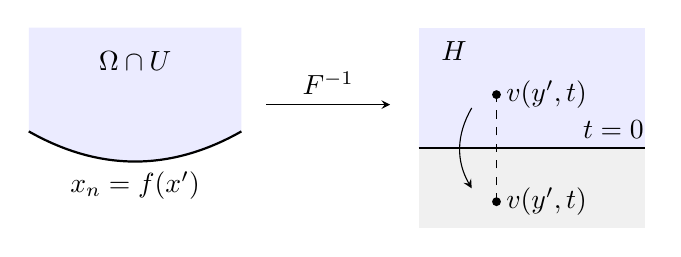
\begin{tikzpicture}[x=.9cm,y=.85cm,>=stealth]
	\fill[blue!8] (0,.25) .. controls (1,-.35) and (2,-.35) .. (3,.25) -- (3,1.8)--(0,1.8)--cycle;
	\draw[thick] (0,.25) .. controls (1,-.35) and (2,-.35) .. (3,.25);
	\node at (1.5,1.3) {\(\Omega\cap U\)};
	\node[below] at (1.5,-.2) {\(x_n=f(x')\)};
	\draw[->] (3.35,.65)--(5.1,.65) node[midway,above] {\(F^{-1}\)};
	\fill[blue!8] (5.5,0) rectangle (8.7,1.8);
	\fill[gray!12] (5.5,-1.2) rectangle (8.7,0);
	\draw[thick] (5.5,0)--(8.7,0);
	\node[above] at (8.25,0) {\(t=0\)};
	\node at (6,1.45) {\(H\)};
	\draw[dashed] (6.6,-.8)--(6.6,.8);
	\fill (6.6,.8) circle (1.6pt) node[right] {\(v(y',t)\)};
	\fill (6.6,-.8) circle (1.6pt) node[right] {\(v(y',t)\)};
	\draw[->] (6.25,.6) to[bend right=30] (6.25,-.6);
\end{tikzpicture}

	\caption[边界展平与反射延拓]{边界展平与反射延拓。左边的图形边界经 \(F^{-1}\) 变为右边的 \(t=0\)；下半空间的值由上半空间对称点的值给定。局部截断使图的侧边不产生新的跳跃。}
	\label{g3:fig:boundary-extension}
\end{figure}

这个定理使有界 \(C^1\) 域满足\cref{g3:def:sobolev-extension-domain}的延拓条件。由\cref{g3:thm:euclidean-sobolev,g3:prop:critical-sobolev,g3:thm:local-morrey}，先对 \(Eu\) 使用全空间估计再限制回来，得到区域上的连续嵌入：当 \(1\le p<n\) 时，\(W^{1,p}(\Omega)\) 嵌入 \(L^{np/(n-p)}(\Omega)\)；当 \(p=n\ge2\) 时，嵌入每个有限 \(L^q\)；当 \(p>n\) 时，有指数 \(1-n/p\) 的连续代表直到边界。\Cref{g3:thm:rellich-domain}同时给出这些嵌入在严格次临界范围内的紧性。一般函数的估计右侧采用完整 \(W^{1,p}\) 范数，因而包含 \(\|u\|_{L^p}\) 项。

\subsection{迹映射的连续性}
\label{g3:subsec:1106:02}
一个 \(L^p(\Omega)\) 等价类可以任意改变边界上的取值，所以不能直接把代表限制到 \(\partial\Omega\)。所需边界值应由内部逼近确定，并且不同逼近必须给出同一结果。一维估计提供了这种唯一性。

\begin{theorem}\label{g3:thm:sobolev-trace}
	设 \(\Omega\subset\mathbb R^n\) 为有界 \(C^1\) 域，\(1\le p<\infty\)，边界测度记为 \(\mathrm dS\)；\(n=1\) 时取端点计数测度。存在唯一有界线性\term[ji yingshe]{迹映射}[trace operator]
	\[
		\operatorname{Tr}:W^{1,p}(\Omega)\longrightarrow L^p(\partial\Omega,\mathrm dS),
	\]
	它在环境光滑函数上等于通常的边界限制。存在 \(h_0>0\) 及 \(C\)，使对 \(0<h<h_0\) 有
	\begin{equation}\label{g3:eq:trace-layer-bound}
		\|\operatorname{Tr}u\|_{L^p(\partial\Omega)}^p
		\le C\left(h^{-1}\|u\|_{L^p(\Omega)}^p
		+h^{p-1}\|\mathrm Du\|_{L^p(\Omega)}^p\right).
	\end{equation}
	若 \(1<p<\infty\)，则对每个 \(\varepsilon>0\)，存在 \(C_\varepsilon\) 使
	\begin{equation}\label{g3:eq:trace-epsilon-bound}
		\|\operatorname{Tr}u\|_{L^p(\partial\Omega)}^p
		\le\varepsilon\|\mathrm Du\|_{L^p(\Omega)}^p
		+C_\varepsilon\|u\|_{L^p(\Omega)}^p.
	\end{equation}
	若 \(u\in W^{1,p}(\Omega)\cap C(\overline\Omega)\)，其迹等于连续代表在边界的值，几乎处处成立。
\end{theorem}
\begin{proof}
	先对平半柱中的光滑函数 \(v(y',t)\) 使用微积分基本公式。对 \(0<t<h\)，有
	\[
		|v(y',0)|^p
		\le2^{p-1}|v(y',t)|^p
		+2^{p-1}t^{p-1}\int_0^t|\partial_t v(y',s)|^p\,\mathrm ds.
	\]
	这里 \(p=1\) 直接用积分三角不等式，其余情形用 Hölder 不等式。对 \(t\in(0,h)\) 取平均，再对 \(y'\) 积分，得到
	\[
		\int|v(y',0)|^p\,\mathrm dy'
		\le2^{p-1}\left(h^{-1}\int_0^h\!\int|v|^p\,\mathrm dy'\mathrm dt
		+h^{p-1}\int_0^h\!\int|\partial_t v|^p\,\mathrm dy'\mathrm dt\right).
	\]
	在每个边界图中令 \(v=(\chi_a u)\circ F\)。表面积元是 \(\sqrt{1+|\mathrm Df|^2}\,\mathrm dy'\)，它与 \(\mathrm dy'\) 一致可比。换元和乘法估计把右侧变成 \(u\) 与 \(\mathrm Du\) 的积分；由 \(\mathrm D\chi_a\) 产生的 \(h^{p-1}\|u\|_p^p\) 项在 \(h<h_0\le1\) 时并入 \(h^{-1}\|u\|_p^p\)。有限求和即得式\eqref{g3:eq:trace-layer-bound}。

	固定一个允许的 \(h\)，便得光滑函数的有界迹估计。由\cref{g3:thm:sobolev-extension-c1}的稠密性，若 \(u_j\to u\) 于 \(W^{1,p}\)，则边界限制 \(u_j|_{\partial\Omega}\) 是 \(L^p(\partial\Omega)\) 中的 Cauchy 列。定义其极限为 \(\operatorname{Tr}u\)。同一估计应用于两个逼近序列之差，证明定义无关；它也证明线性、有界性及唯一性，并使薄层估计延续到全部 \(u\)。当 \(p>1\) 时，选 \(h\) 使 \(Ch^{p-1}\le\varepsilon\)，即得式\eqref{g3:eq:trace-epsilon-bound}。

	若 \(u\) 在闭包连续，前一定理中的反射、截断和有限求和给出一个连续紧支延拓。它的卷积同时在闭包上一致收敛到 \(u\)，又在 \(W^{1,p}\) 中收敛。因此其边界限制的 \(L^p\) 极限就是 \(u|_{\partial\Omega}\)，证明最后一项。
\end{proof}
\symidx{\(\operatorname{Tr}u\)：Sobolev 函数或截面的边界迹}

薄层估计还显示了尺度。对一个固定的 \(C^1\) 域 \(\Omega_1\) 及 \(\Omega_R=R\Omega_1\)，换元 \(x=Ry\) 给出
\[
	\|\operatorname{Tr}u\|_{L^p(\partial\Omega_R)}^p
	\le C\left(R^{-1}\|u\|_{L^p(\Omega_R)}^p
	+R^{p-1}\|\mathrm Du\|_{L^p(\Omega_R)}^p\right).
\]
左侧在缩放中有 \(n-1\) 维的因子，两个右侧项恰有相同尺度。

\ProseParagraphBreak

\(p=1\) 时，式\eqref{g3:eq:trace-layer-bound}仍成立，但梯度前的系数不随 \(h\downarrow0\) 消失。例如在一个平边界片取非零光滑紧支 \(\psi(y')\)，再取 \(\eta(0)=1\)、支集位于 \([0,1)\) 的光滑函数，令 \(v_\delta(y',t)=\psi(y')\eta(t/\delta)\)。它的内部 \(L^1\) 范数趋零，\(\|\mathrm Dv_\delta\|_{L^1}\) 保持有界，而边界迹恒为 \(\psi\)。选足够小的固定 \(\varepsilon\) 就能看出，一般不能把式\eqref{g3:eq:trace-epsilon-bound}中的任意小系数结论扩展到 \(p=1\)。

\begin{proposition}\label{g3:prop:weak-boundary-integration}
	设 \(\Omega\subset\mathbb R^n\) 为有界 \(C^1\) 域，\(1\le p<\infty\)，\(u\in W^{1,p}(\Omega)\)，\(\phi\) 在 \(\overline\Omega\) 的邻域中光滑。若 \(\nu\) 为外单位法向，则
	\begin{equation}\label{g3:eq:weak-boundary-integration}
		\int_\Omega u\,\partial_i\phi\,\mathrm dx
		=-\int_\Omega(\partial_i u)\phi\,\mathrm dx
		+\int_{\partial\Omega}(\operatorname{Tr}u)\phi\nu_i\,\mathrm dS.
	\end{equation}
\end{proposition}
\begin{proof}
	先取光滑 \(u\)。在图形区域 \(x_n>f(x')\) 内，沿 \(x_n\) 积分给出下端点项；切向积分时，对变动下限 \(f(x')\) 求导，给出 \(\partial_i f\) 的因子。这恰是
	\[
		\nu\,\mathrm dS=(\mathrm Df,-1)\,\mathrm dx'
	\]
	的各分量。用单位分解求和，内部片无边界项，单位分解的导数因其总和为一而相消，得到光滑函数的公式。最后用贴边光滑函数在 \(W^{1,p}\) 中逼近 \(u\)。区域和边界测度都有限，内部两项按 \(L^p\) 收敛，边界项按迹的连续性收敛，故公式成立。
\end{proof}

\subsection{零边界 Sobolev 空间}
\label{g3:subsec:1106:03}
\(W_0^{1,p}(\Omega)\) 按定义是 \(C_c^\infty(\Omega)\) 的 \(W^{1,p}\) 闭包。它首先描述可逼近性。下面证明，在规则边界上，这个闭包恰好实现零边界值；零延拓是否产生额外边界导数是两种描述之间的联系。

\begin{theorem}\label{g3:thm:zero-trace-characterization}
	设 \(\Omega\subset\mathbb R^n\) 为有界 \(C^1\) 域，\(1\le p<\infty\)，\(u\in W^{1,p}(\Omega)\)。记 \(\widetilde u\) 为 \(u\) 在 \(\mathbb R^n\setminus\Omega\) 上补零的函数。则以下条件等价：
	\begin{equivalences}
		\item \(u\in W_0^{1,p}(\Omega)\)；
		\item \(\operatorname{Tr}u=0\)；
		\item \(\widetilde u\in W^{1,p}(\mathbb R^n)\)。
	\end{equivalences}
	此时 \(\partial_i\widetilde u=\widetilde{\partial_i u}\)，几乎处处成立。
\end{theorem}
\begin{proof}
	若 \(u\in W_0^{1,p}\)，用紧支于 \(\Omega\) 的光滑函数逼近。它们的迹都是零，故由连续性得到第二项；它们的零延拓及其导数在全空间同样是 Cauchy 列，故也得到第三项及所列导数公式。

	若 \(\operatorname{Tr}u=0\)，对任意 \(\phi\in C_c^\infty(\mathbb R^n)\)，式\eqref{g3:eq:weak-boundary-integration}成为
	\[
		\int_{\mathbb R^n}\widetilde u\,\partial_i\phi\,\mathrm dx
		=-\int_{\mathbb R^n}\widetilde{\partial_i u}\,\phi\,\mathrm dx.
	\]
	右侧由一个 \(L^p\) 函数给出，所以零延拓属于 \(W^{1,p}\)，并具有指定弱导数。

	现在从第三项构造内部紧支逼近。这一步既适用于 \(p>1\)，也适用于 \(p=1\)。用前述有限单位分解将 \(u\) 分成内部项与边界项。内部项离边界有正距离，直接卷积即可。对边界项，将其零延拓通过展平坐标拉回，得到一个紧支 \(w\in W^{1,p}(\mathbb R^n)\)，且 \(w=0\) 于 \(t<0\)。令
	\[
		w_\delta(y',t)=w(y',t-\delta),\qquad \delta>0.
	\]
	这将支集向区域内部移动，因而 \(w_\delta=0\) 于 \(t<\delta\)。由 \(L^p\) 平移连续性，函数及其全部一阶弱导数都收敛，所以 \(w_\delta\to w\) 于 \(W^{1,p}\)。再取卷积半径 \(\varepsilon_\delta<\delta/2\)，使卷积误差趋零。所得光滑函数的支集仍在 \(t>\delta/2\)，并可使其始终留在原来较大的坐标图内。

	将这些函数送回原坐标，得到离 \(\partial\Omega\) 有正距离的紧支 \(C^1\) 函数。若边界图只有 \(C^1\)，再对每个这样的函数在原 Euclid 坐标中作一次足够小半径的卷积，便得到 \(C_c^\infty(\Omega)\) 函数，且误差可任意小。换元估计保证此前的收敛仍为 \(W^{1,p}\) 收敛。有限个局部项相加，就得到逼近 \(u\) 的内部紧支光滑序列，证明第一项。
\end{proof}

例如区间上的常函数一属于 \(W^{1,p}(0,1)\)，但不属于 \(W_0^{1,p}(0,1)\)。它的零延拓是区间的示性函数，分布导数为 \(\delta_0-\delta_1\)，并非 \(L^p\) 函数。边界跳跃恰对应刚才分部积分中没有消失的边界项。

\ProseParagraphBreak

对非零给定边界数据，若已选定一个提升 \(g\in W^{1,p}(\Omega)\)，则所有满足 \(\operatorname{Tr}u=\operatorname{Tr}g\) 的函数恰为
\[
	g+W_0^{1,p}(\Omega).
\]
这是迹的线性与核的刻画直接给出的仿射空间。以后构造弱解时，减去 \(g\) 就把边界条件化为零边界条件。

\subsection{边界正则性的作用}
\label{g3:subsec:1106:04}
前面的常数来自有限个图的大小、展平映射及逆映射的导数、表面积元与单位分解。对一族区域，如果这些量一致受控，构造就给出一致的延拓与迹估计。仅知道各个区域分别有光滑边界，并不能使这些常数自动一致。

\begin{proposition}\label{g3:prop:sobolev-boundary-bundles}
	设 \((M,g)\) 为紧的光滑 \(n\) 维带边界黎曼流形，\(E\to M\) 为带光滑纤维度量及相容联络的有限秩实或复向量丛，\(1\le p<\infty\)。则存在有界线性映射
	\[
		\operatorname{Tr}:W^{1,p}(M;E)\longrightarrow
		L^p(\partial M;E|_{\partial M}),
	\]
	它延拓光滑截面的边界限制，且
	\[
		\ker\operatorname{Tr}=W_0^{1,p}(M;E),
	\]
	右侧为内部紧支光滑截面的闭包。式\eqref{g3:eq:trace-layer-bound}和 \(p>1\) 时的式\eqref{g3:eq:trace-epsilon-bound}也成立，将 \(\mathrm D\) 换为 \(\nabla\)、体积及表面积换为诱导的密度即可。相应的一阶嵌入范围为：
	\begin{enumerate}
		\item 当 \(1\le p<n\) 时，连续嵌入 \(L^q(M;E)\)，\(1\le q\le np/(n-p)\)；严格小于该上端点时嵌入为紧。
		\item 当 \(p=n\ge2\) 时，对每个 \(1\le q<\infty\)，到 \(L^q(M;E)\) 的嵌入为紧，因而连续。
		\item 当 \(p>n\) 时，连续嵌入 \(C^{0,\alpha}(M;E)\)，\(\alpha=1-n/p\)；到 \(C^{0,\beta}(M;E)\) 的嵌入在 \(0\le\beta<\alpha\) 时为紧，这里 \(\beta=0\) 表示一致范数。
		\item 当 \(n=p=1\) 时，连续嵌入 \(C^0(M;E)\)，并紧嵌入每个有限 \(L^q(M;E)\)。
	\end{enumerate}
	Hölder 范数按有限坐标图与丛标架定义。
\end{proposition}
\begin{proof}
	取有限个内部图及边界半空间图，并在各图内选择光滑丛标架。将截面乘以单位分解后逐分量反射、卷积，得到直到边界都光滑的逼近截面。局部范数与 \(\sum(|u^a|^p+|\mathrm Du^a|^p)\) 的积分等价：体积密度和纤维度量有正的上下界，协变导数与普通导数相差有界联络系数乘以截面的零阶项。

	各分量的边界迹因而满足一致的有限图估计。在两组标架的交集，分量由一个光滑可逆矩阵联系；在光滑截面上，取边界值与该矩阵的限制相容。再用逼近与乘法连续性取极限，这个相容关系保留，所以局部迹粘成 \(E|_{\partial M}\) 的截面，与标架及单位分解无关。标量证明中的分部积分、零延拓和向内平移逐分量进行，证明核正是内部紧支光滑截面的闭包。

	对每个局部项用半空间延拓，再使用欧氏 Sobolev 与 Rellich 结论，便得到相应的连续嵌入与紧嵌入；紧性只需对有限个图依次取子列。范数等价负责把分量收敛还原成截面收敛。迹的薄层估计也逐图求和；联络及截断引入的零阶项并入已有零阶项，便得到所述两种估计。
\end{proof}

\begin{proposition}\label{g3:prop:higher-order-boundary-extension}
	设 \(k\ge1\) 为整数，\(\Omega\subset\mathbb R^n\) 是有界 \(C^k\) 域，\(1\le p<\infty\)。则存在有界线性延拓
	\[
		E_k:W^{k,p}(\Omega)\longrightarrow W^{k,p}(\mathbb R^n),
	\]
	其支集包含于一个固定紧集。该构造的常数由有限边界图及逆图直到 \(k\) 阶的导数和相应截断函数控制。
\end{proposition}
\begin{proof}
	半空间上的偶反射一般不能保留二阶弱导数，例如 \(v(t)=t\) 的偶反射为 \(|t|\)，其一阶导数在零处跳跃。为使直到 \(k-1\) 阶的法向导数匹配，选择 \(c_1,\ldots,c_k\) 满足
	\[
		\sum_{j=1}^k c_j(-j)^\ell=1,
		\qquad 0\le\ell\le k-1.
	\]
	这些系数存在且唯一：系数矩阵可逆，因为次数不超过 \(k-1\) 的多项式若在 \(-1,\ldots,-k\) 都为零，就恒为零。对在闭半空间光滑的 \(v\)，在 \(t<0\) 定义
	\[
		(E_kv)(y',t)=\sum_{j=1}^k c_jv(y',-jt),
	\]
	在 \(t\ge0\) 保留原值。上述等式使所有总阶数小于 \(k\) 的导数在两侧相接。逐次分部积分时，直到第 \(k\) 次求导都没有边界跳跃项。每项的 \(\ell\) 次法向导数只多出 \((-j)^\ell\)，再以 \(s=-jt\) 换元，便得到 \(W^{k,p}\) 范数界。

	这里所用的闭半空间光滑稠密性也可在任意整数阶直接建立。先在远处截断，随后将 \(v(y',t)\) 替换为 \(v(y',t+\delta)\)。后者在 \(t>-\delta\) 已有定义；其各阶弱导数在 \(H\) 上趋于原导数，这是将这些 \(L^p(H)\) 导数各自补零后应用平移连续性的结果。再在半径小于 \(\delta/2\) 内卷积，得到闭半空间附近光滑的函数；对所有不超过 \(k\) 阶的导数同时选择足够小的卷积半径，就得到 \(W^{k,p}(H)\) 逼近。因此前述有界反射算子可连续延拓到全部 \(W^{k,p}(H)\)。

	对一般 \(C^k\) 域，使用与一阶情形相同的有限覆盖、单位分解及展平。反复使用链式法则，\(C^k\) 图及逆图的有界导数控制全部不超过 \(k\) 阶的范数。将半空间延拓限制在足够薄的较大图内、乘截断后送回并求和，就得到所需算子与固定紧支集。
\end{proof}

这个证明说明了所选展平构造为何要求相应阶数的导数控制。\(C^1\) 边界也不是一阶延拓存在的必要条件：矩形的角点不满足 \(C^1\) 图形条件，但逐个坐标反射、再乘固定截断函数，仍给出一阶有界延拓。判断边界正则性时，要检查实际能否作有界的局部变换与拼接。

\begin{example}\label{g3:exm:slit-domain-traces}
	考虑去掉一条半径的单位圆盘
	\[
		\Omega=\{(r\cos\theta,r\sin\theta):0<r<1,\ 0<\theta<2\pi\}.
	\]
	取 \(\chi\in C_c^\infty((1/4,3/4))\)，且在一个较小区间上等于一，定义 \(u(r,\theta)=\chi(r)\theta\)。函数及其一阶导数在 \(\Omega\) 上有界，所以 \(u\in W^{1,p}(\Omega)\) 对每个有限 \(p\) 成立。裂缝的上侧边界值为零，下侧为 \(2\pi\chi(r)\)，两侧都来自各自半邻域中的光滑限制。

	不存在把这个 \(u\) 延拓到整个圆盘的 \(W^{1,p}\) 函数。事实上，对裂缝中 \(\chi=1\) 的一段，几乎每条横穿裂缝的竖直线在两侧都有相差 \(2\pi\) 的极限。若延拓属于 \(W^{1,p}\)，绝对连续切片判据要求同一条线上的代表跨过裂缝连续，矛盾。裂缝作为平面中的点集只有一份，但域内逼近有两侧；在这种区域上，边界值必须保留所从属的一侧。
\end{example}
% 纲要条目排为编号小节标题，并进入目录与书签；说明段仍保留于纲要注释中。


\begin{chaptersummary}
弱导数由分部积分确定，局部平滑与坐标变换保证这一概念能够用于流形及向量丛。整数阶 Sobolev 范数把截面与各阶弱协变导数放进一组 \(L^p\) 空间，闭图关系给出完备性；在 \(1<p<\infty\) 时，积分对偶和反射性给出有界序列的弱收敛子列。光滑稠密性、截断与链式法则使这些空间能够承接微分方程中的测试和非线性运算。

\ProseParagraphBreak

Sobolev 嵌入把导数可积性换成更高的函数可积性，Morrey 估计进一步产生连续代表。临界指数与高阶端点须按维数和导数阶数判断。Poincaré 不等式通过边界条件、均值或平行截面投影去掉导数的核；其常数记录着尺度与连通区域之间的联系。Rellich 紧性则把平移控制和尾部控制化为有限近似，在严格低于临界指数处得到强收敛子列。

\ProseParagraphBreak

边界展平与反射提供延拓，法向的一维微积分给出连续迹。对有界 \(C^1\) 域，零迹恰好刻画内部紧支光滑函数的 \(W^{1,p}\) 闭包，也恰好保证补零后仍有全局一阶弱导数；高阶延拓还要匹配更多阶的边界导数。下一章将在这些空间上建立弱椭圆方程，先由能量估计获得解，再用局部与边界正则性恢复更强的微分性质。
\end{chaptersummary}

\BookExercises

\begin{exercise}\label{g3:ex:circle-sawtooth-weak}
	在周长为 \(L>0\) 的圆周 \(S^1_L=\mathbb R/L\mathbb Z\) 上，用 \([0,L)\) 的代表定义 \(u([x])=x\)。以周期光滑测试函数定义分布导数，求 \(\partial_xu\)，并判断 \(u\) 是否属于 \(W^{1,p}(S^1_L)\)，\(1\le p\le\infty\)。
\end{exercise}
\begin{solution}
	对周期光滑函数 \(\varphi\)，分部积分给出
	\[
		-\int_0^L x\varphi'(x)\,\mathrm dx
		=\int_0^L\varphi(x)\,\mathrm dx-L\varphi(0).
	\]
	因此 \(\partial_xu=1-L\delta_{[0]}\)。该函数有界，属于每个 \(L^p\)，但其导数包含点质量。由\cref{g3:exm:point-distribution}，点质量不能由局部可积函数表示，故它不属于任何上述 \(W^{1,p}\)。在开区间 \((0,L)\) 中只看到导数一，圆周的端点识别却引入了一个大小为 \(-L\) 的跳跃。
\end{solution}

\begin{exercise}\label{g3:ex:weighted-interval-weak-laplacian}
	设 \(a\in C^\infty([0,1])\) 且 \(a>0\)，在区间上取度量 \(g=a(x)^2\mathrm dx^2\)。写出标量 \(H^1\) 范数与弱 Laplace 算子。再设 \(u\in H^1(0,1)\)、\(f\in L^1_{\mathrm{loc}}(0,1)\)，以 \(y=\int_0^x a(t)\,\mathrm dt\) 换坐标，证明这一范数及弱方程 \(\Delta_gu=f\) 分别变为长度为 \(\ell=\int_0^1a\) 的普通区间上的标准 \(H^1\) 范数及 \(-\partial_y^2\widetilde u=\widetilde f\)。
\end{exercise}
\begin{solution}
	体积密度为 \(a\,\mathrm dx\)，而 \(|\mathrm du|_g^2=a^{-2}|u'|^2\)，所以
	\[
		\|u\|_{H^1(g)}^2=\int_0^1\left(a|u|^2+a^{-1}|u'|^2\right)\,\mathrm dx.
	\]
	弱方程表示对每个内部紧支光滑 \(\varphi\) 有
	\[
		\int_0^1a^{-1}u'\varphi'\,\mathrm dx=\int_0^1fa\varphi\,\mathrm dx.
	\]
	因此在分布意义下 \(\Delta_gu=-a^{-1}\partial_x(a^{-1}u')\)。换元满足 \(\mathrm dy=a\,\mathrm dx\)、\(u'=a\partial_y\widetilde u\)，两个积分变成
	\[
		\int_0^\ell\left(|\widetilde u|^2+|\partial_y\widetilde u|^2\right)\,\mathrm dy,
		\qquad
		\int_0^\ell(\partial_y\widetilde u)(\partial_y\widetilde\varphi)\,\mathrm dy
		=\int_0^\ell\widetilde f\widetilde\varphi\,\mathrm dy.
	\]
	\(a\) 有正下界，换元及逆换元的一阶导数有界，故\cref{g3:prop:weak-coordinate-change}保证这些计算也适用于弱导数。最后的恒等式正是所述非负 Laplace 约定下的方程。
\end{solution}

\begin{exercise}\label{g3:ex:noncompact-connection-sobolev}
	在 \(\mathbb R\times\mathbb C\) 上取标准底度量和纤维 Hermitian 度量，比较两个相容联络
	\[
		\nabla=\mathrm d,\qquad\nabla'=\mathrm d+\mathrm i x\,\mathrm dx.
	\]
	设 \(1\le p<\infty\)，令 \(a=1/p+1/2\)、\(s(x)=(1+x^2)^{-a/2}\)。证明 \(s\in W^{1,p}_\nabla\)，但 \(s\notin W^{1,p}_{\nabla'}\)。解释这为何不与紧流形上的联络无关性矛盾。
\end{exercise}
\begin{solution}
	联络一形式 \(\mathrm ix\,\mathrm dx\) 是反 Hermitian 的，故 \(\nabla'\) 也保持标准纤维度量。无穷远处 \(|s|\) 与 \(|x|^{-a}\) 可比，\(|s'|\) 与 \(|x|^{-a-1}\) 可比；由于 \(ap=1+p/2>1\)，两者的 \(p\) 次幂都可积。因此 \(s\in W^{1,p}_\nabla\)。

	由于 \(s,s'\) 为实值，
	\[
		|\nabla's|^2=|s'+\mathrm ixs|^2=|s'|^2+x^2s^2.
	\]
	\(|xs|^p\) 在无穷远处与 \(|x|^{p(1-a)}\) 可比，其可积性要求 \((a-1)p>1\)；这里 \((a-1)p=1-p/2<1\)，所以不可积。两个联络之差的系数 \(x\) 无界，紧流形证明所用的统一系数界不成立。它们在每个固定紧区间上仍定义等价范数。
\end{solution}

\begin{exercise}\label{g3:ex:weak-strong-oscillation}
	在 \(S^1_{2\pi}\) 上令 \(u_j(x)=j^{-1}\sin(jx)\)，\(1<p<\infty\)。证明 \(u_j\to0\) 于每个有限 \(L^q\) 及一致范数，\(u_j\rightharpoonup0\) 于 \(W^{1,p}\)，但它没有 \(W^{1,p}\) 强收敛子列。
\end{exercise}
\begin{solution}
	由 \(\|u_j\|_\infty\le j^{-1}\)，得到全部所述零阶强收敛。一阶导数为 \(u_j'=\cos(jx)\)，其 \(L^p\) 范数恒等于 \(\|\cos x\|_{L^p(0,2\pi)}>0\)。若某子列在 \(W^{1,p}\) 中强收敛，零阶极限只能为零，导数范数也应趋零，矛盾。

	对周期光滑测试函数 \(\psi\)，分部积分给出
	\[
		\left|\int_0^{2\pi}\psi(x)\cos(jx)\,\mathrm dx\right|
		\le j^{-1}\|\psi'\|_{L^1}.
	\]
	光滑函数在 \(L^{p'}\) 中稠密，而 \(\cos(jx)\) 的 \(L^p\) 范数一致有界，故这一配对趋零对所有 \(L^{p'}\) 测试函数成立。因此 \((u_j,u_j')\rightharpoonup(0,0)\) 于 \(L^p\times L^p\)。\(W^{1,p}\) 是这个乘积空间的闭子空间，每个有界线性泛函都可按\cref{g3:lem:bounded-functional-extension}延拓，故这正给出 \(W^{1,p}\) 中的弱收敛。高频振荡可以保留导数范数，同时使每个固定测试配对趋零。
\end{solution}

\begin{exercise}\label{g3:ex:bundle-modulus-sharpness}
	在 \(S^1_{2\pi}\) 的平凡复线丛上取平坦联络。令 \(s_j(x)=e^{\mathrm ijx}\)。计算 \(\||s_j|\|_{W^{1,p}}\) 和 \(\|\nabla s_j\|_{L^p}\)，\(1\le p<\infty\)。说明模长估计不能反向控制截面的导数。再设在连通开集 \(U\subset\mathbb R^n\) 上有光滑表示 \(s=\rho e^{\mathrm i\theta}\)，其中 \(\rho>0\)、\(\theta\) 实值。证明模长不等式处处取等号，当且仅当 \(\theta\) 为常数。
\end{exercise}
\begin{solution}
	\(|s_j|=1\)，所以 \(\||s_j|\|_{W^{1,p}}=(2\pi)^{1/p}\)；而 \(|\nabla s_j|=j\)，故 \(\|\nabla s_j\|_p=j(2\pi)^{1/p}\)。模长不记录相位变化，因此不存在由模长的这个范数统一控制截面导数的反向估计。

	对第二问，直接计算得到
	\[
		\mathrm ds=e^{\mathrm i\theta}(\mathrm d\rho+\mathrm i\rho\,\mathrm d\theta),
		\qquad |\mathrm ds|^2=|\mathrm d\rho|^2+\rho^2|\mathrm d\theta|^2.
	\]
	由于 \(\rho>0\)，模长不等式处处取等号等价于 \(\mathrm d\theta=0\)。连通开集中的两点可以用有限条线段连接，沿每条线段应用微积分基本定理，便知这一条件等价于 \(\theta\) 为常数。
\end{solution}

\begin{exercise}\label{g3:ex:radial-sobolev-threshold}
	设 \(n\ge2\)、\(1\le p<n\)，\(\eta\in C_c^\infty(B_1(0))\) 在 \(B_{1/2}(0)\) 上等于一。对 \(a>0\)，令 \(u_a(x)=\eta(x)|x|^{-a}\)。求 \(u_a\in W^{1,p}(B_1)\) 的充要条件，以及 \(u_a\in L^q(B_1)\)（\(1\le q<\infty\)）的条件。由此说明在固定球中，\(W^{1,p}\) 嵌入的上限指数 \(p^*=np/(n-p)\) 不能提高。
\end{exercise}
\begin{solution}
	在零点以外，\(|\mathrm Du_a|=a|x|^{-a-1}\) 当 \(|x|<1/2\)。极坐标积分说明
	\[
		\int_0^{1/2}r^{n-1-aq}\,\mathrm dr<\infty
		\quad\Longleftrightarrow\quad aq<n,
	\]
	而梯度的 \(p\) 次幂可积当且仅当 \((a+1)p<n\)。等号时积分为 \(\int\mathrm dr/r\)，仍发散。

	若 \((a+1)p<n\)，则 \(a<n-1\)。在穿孔球上分部积分，内边界项至多为常数乘 \(\varepsilon^{n-1-a}\)，故趋零；经典导数于是给出全球弱导数，且 \(u_a\in L^p\)。反过来，若 \(u_a\) 属于 \(W^{1,p}\)，在任何避开零点的开集上，其弱导数必须等于已算出的经典导数，因此 \((a+1)p<n\) 必要。这得到充要条件。

	给定 \(q>p^*\)，有 \(n/q<n/p-1\)，故可取
	\(n/q\le a<n/p-1\)。此时 \(u_a\in W^{1,p}\) 却不在 \(L^q\)。由于它支于球内部，前述局部卷积也表明它属于 \(W_0^{1,p}(B_1)\)，所以即使加入零边界条件也不能提高最大指数。所有 \(a>0\) 的函数都在零附近无界，亦给出 \(L^\infty\) 失败。
\end{solution}

\begin{exercise}\label{g3:ex:morrey-sharp-exponent}
	设 \(n<p<\infty\)，令 \(\alpha=1-n/p\)。取 \(\varphi\in C_c^\infty(B_1(0))\)，满足 \(\varphi(0)=1\)，并定义
	\[
		u_\varepsilon(x)=\varepsilon^\alpha\varphi(x/\varepsilon),
		\qquad 0<\varepsilon<1/3.
	\]
	证明 \(u_\varepsilon\) 在 \(W^{1,p}(B_1)\) 中有界，而且一致趋于零；但对任何 \(\alpha<\beta\le1\)，\([u_\varepsilon]_{C^{0,\beta}(B_1)}\to\infty\)。说明这对 Morrey 指数的意义。
\end{exercise}
\begin{solution}
	换元给出
	\[
		\|u_\varepsilon\|_p=\varepsilon^{\alpha+n/p}\|\varphi\|_p
		=\varepsilon\|\varphi\|_p,\qquad
		\|\mathrm Du_\varepsilon\|_p=\varepsilon^{\alpha-1+n/p}\|\mathrm D\varphi\|_p
		=\|\mathrm D\varphi\|_p.
	\]
	且 \(\|u_\varepsilon\|_\infty=\varepsilon^\alpha\|\varphi\|_\infty\to0\)。另一方面，在 \(0\) 与 \(2\varepsilon e_1\) 两点的函数值分别为 \(\varepsilon^\alpha\)、零，因而
	\[
		[u_\varepsilon]_{C^{0,\beta}(B_1)}\ge2^{-\beta}\varepsilon^{\alpha-\beta}\longrightarrow\infty.
	\]
	因此原 Sobolev 范数不能统一控制任何更大的 Hölder 指数。每个函数自身虽光滑，这列函数在不断缩小的区域中仍有比 \(\beta\) 次幂更强的振荡；一致收敛也不能给出高阶模连续性的统一界。
\end{solution}

\begin{exercise}\label{g3:ex:sobolev-multiplication-threshold}
	设 \((M^n,g)\) 为紧、光滑、无边界黎曼流形，\(n<p<\infty\)。用本章乘法代数的范数估计证明，对每个实值 \(u\in W^{1,p}(M)\)，指数级数在 \(W^{1,p}\) 中收敛，且
	\[
		e^u-1\in W^{1,p}(M),\qquad
		\|e^u-1\|_{W^{1,p}}\le\|u\|_{W^{1,p}}\exp\bigl(C\|u\|_{W^{1,p}}\bigr).
	\]
	证明其弱导数为 \(e^u\,\mathrm du\)。再在 \(n\ge2\)、\(1\le p<n\) 的情形，构造支于一个坐标球的 \(u\in W^{1,p}(M)\)，使 \(u^2\notin W^{1,p}(M)\)。
\end{exercise}
\begin{solution}
	令 \(C\ge1\) 为\cref{g3:cor:sobolev-multiplication-algebra}中 \(k=1\) 的常数，记 \(A=\|u\|_{W^{1,p}}\)。归纳得到 \(\|u^j\|_{W^{1,p}}\le C^{j-1}A^j\)，故
	\[
		\sum_{j=1}^\infty\left\|\frac{u^j}{j!}\right\|_{W^{1,p}}
		\le A\sum_{j=1}^\infty\frac{(CA)^{j-1}}{j!}\le A e^{CA}.
	\]
	由完备性，该级数在 \(W^{1,p}\) 中收敛。\cref{g3:thm:compact-bundle-sobolev}给出到 \(C^0\) 的连续嵌入，所以它也一致收敛；逐点普通指数级数将极限识别为 \(e^u-1\)。对部分和使用弱乘积公式，其导数为
	\[
		\left(\sum_{j=1}^N\frac{u^{j-1}}{(j-1)!}\right)\mathrm du.
	\]
	括号中的级数一致趋于 \(e^u\)，乘 \(L^p\) 的 \(\mathrm du\) 后在 \(L^p\) 中收敛，故弱导数正是所述公式。

	当 \(p<n\) 时，记 \(A=n/p-1>0\)，选择
	\[
		\frac A2<a<\min\left\{A,\frac n{2p}\right\}.
	\]
	右端严格大于左端，故可选到。取坐标球内的紧支截断，定义 \(u=\eta(x)|x|^{-a}\)，在球外补零。度量及体积密度在截断支集上与 Euclid 数据一致可比，\cref{g3:ex:radial-sobolev-threshold}的计算给出 \(u\in W^{1,p}(M)\)。同时 \(2ap<n\)，故 \(u^2\in L^p\)；但 \((2a+1)p>n\)，其在穿孔小球中的经典梯度不属于 \(L^p\)。若存在全局 \(L^p\) 弱导数，它在这个穿孔区域中必须与该梯度一致，产生矛盾。因此乘法闭性确实失败。
\end{solution}

\begin{exercise}\label{g3:ex:poincare-positive-measure-anchor}
	设 \((M,g)\) 为连通、紧且无边界的光滑黎曼流形，\(1\le p<\infty\)，其零均值 Poincaré 常数为 \(C_P\)。设可测集 \(A\subset M\) 满足 \(\operatorname{Vol}(A)\ge a>0\)。证明：若 \(u\in W^{1,p}(M)\) 且 \(u=0\) 几乎处处于 \(A\)，则
	\[
		\|u\|_{L^p(M)}\le C_P\left[1+\left(\frac{\operatorname{Vol}(M)}a\right)^{1/p}\right]\|\mathrm du\|_{L^p(M)}.
	\]
	再解释将“正测度集上为零”换成“某一点取值为零”时，在 \(n=\dim M\ge2\)、\(p\le n\) 的一般 Sobolev 类中为什么需要重新定义条件。
\end{exercise}
\begin{solution}
	令 \(c=u_M\)。在 \(A\) 上有 \(u-c=-c\)，故
	\[
		|c|a^{1/p}\le\|u-c\|_{L^p(A)}\le C_P\|\mathrm du\|_{L^p(M)}.
	\]
	由三角不等式，
	\[
		\|u\|_p\le\|u-c\|_p+|c|\operatorname{Vol}(M)^{1/p},
	\]
	代入前式即得所求常数。

	Sobolev 元素是几乎处处相等的函数类，改变一个点的取值不改变该元素，也不改变弱导数。若尚未通过连续代表或其他附加结构定义点值，“某一点为零”可由任意函数通过修改零测集实现，因而不能消除常数核。\(p>n\) 时 Morrey 连续代表提供了真正的点值，才可另行讨论以点为锚的估计。
\end{solution}

\begin{exercise}\label{g3:ex:product-poincare-optimal}
	设 \(M,N\) 为正维、连通、紧且无边界的光滑黎曼流形。令 \(C_M,C_N\) 分别为 \(L^2\) 零均值 Poincaré 不等式的最佳常数。证明乘积度量下的最佳常数满足
	\[
		C_{M\times N}=\max\{C_M,C_N\}.
	\]
	证明中不使用 Laplace 特征函数展开。
\end{exercise}
\begin{solution}
	对光滑函数 \(u(x,y)\)，令 \(v(y)=\operatorname{Vol}(M)^{-1}\int_Mu(x,y)\mu_M(x)\)，\(c=u_{M\times N}\)。对每个 \(y\)，\(u-v\) 在 \(M\) 上均值为零，所以 \(u-v\) 与仅依赖 \(y\) 的 \(v-c\) 在乘积 \(L^2\) 内积中正交。因此
	\[
		\|u-c\|_2^2=\|u-v\|_2^2+\|v-c\|_2^2.
	\]
	对第一项逐个 \(M\) 纤维应用不等式，得 \(\|u-v\|_2^2\le C_M^2\|\mathrm d_Mu\|_2^2\)。对第二项在 \(N\) 上应用不等式，并用积分平均的凸性，得
	\[
	\begin{aligned}
		\|v-c\|_{L^2(M\times N)}^2
		&\le C_N^2\operatorname{Vol}(M)\int_N|\mathrm d_Nv|^2\mu_N\\
		&\le C_N^2\|\mathrm d_Nu\|_{L^2(M\times N)}^2.
	\end{aligned}
	\]
	乘积度量使两种梯度平方相加，因而 \(C_{M\times N}\le\max\{C_M,C_N\}\)。光滑稠密性将此估计推广到 \(W^{1,2}\)。反过来，依次取只依赖 \(x\) 或只依赖 \(y\) 的非恒定函数，乘积体积因子在函数范数与梯度范数的比值中抵消，故最佳常数至少分别为 \(C_M,C_N\)。
\end{solution}

\begin{exercise}\label{g3:ex:quantitative-sobolev-finite-net}
	设 \(Q=(0,1)^n\)、\(1\le p<\infty\)，并令
	\[
		\mathcal F=\{u\in W^{1,p}(Q;\mathbb R):u_Q=0,\ \|\mathrm D u\|_{L^p(Q)}\le1\}.
	\]
	把 \(Q\) 分成 \(m^n\) 个边长 \(1/m\) 的小立方体，在每个小立方体上以平均值代替 \(u\)，所得算子记为 \(A_m\)。证明
	\[
		\|u-A_mu\|_{L^p(Q)}\le\frac{2^{n/p}\sqrt n}{m}.
	\]
	再证明存在只依赖 \(n,p\) 的常数 \(C\ge2\)，使 \(0<\varepsilon<1\) 时，\(\mathcal F\) 在 \(L^p(Q)\) 中有一个精度 \(\varepsilon\) 的有限近似集，其点数至多为
	\[
		\exp\!\left(C\varepsilon^{-n}\log\frac C\varepsilon\right).
	\]
	近似集的元素允许为分块常值函数。
\end{exercise}
\begin{solution}
	每个小立方体直径为 \(\sqrt n/m\)。由\cref{g3:prop:poincare-convex-mean}，将各块误差的 \(p\) 次方相加，立即得到第一式。对整个 \(Q\) 使用同一命题，还知 \(\|u\|_p\le C_0=2^{n/p}\sqrt n\)。

	对体积为 \(m^{-n}\) 的任一小块 \(Q_\nu\)，Hölder 不等式给出
	\[
		|u_{Q_\nu}|\le m^{n/p}\|u\|_{L^p(Q_\nu)}\le C_0m^{n/p}.
	\]
	取 \(m=\lceil2C_0/\varepsilon\rceil\)，使平均化误差至多为 \(\varepsilon/2\)。在区间 \([-C_0m^{n/p},C_0m^{n/p}]\) 上取间距不超过 \(\varepsilon\) 的等距刻度，把每个块平均值替换成最近刻度值。各点误差至多为 \(\varepsilon/2\)，而 \(|Q|=1\)，所以新增 \(L^p\) 误差也至多为 \(\varepsilon/2\)。

	每块可选刻度数至多为 \(2+2C_0m^{n/p}/\varepsilon\)，全部分块常值函数数目因而至多为
	\[
		\left(2+\frac{2C_0m^{n/p}}\varepsilon\right)^{m^n}.
	\]
	由于 \(m\le C_1/\varepsilon\)，对上式取对数并吸收只依赖 \(n,p\) 的常数，即得题设上界。这是一个明确的近似规模估计，未断言该数量级最优。
\end{solution}

\begin{exercise}\label{g3:ex:weak-and-strong-sobolev-limits}
	设 \((M^n,g)\) 为紧且无边界的光滑黎曼流形。
	\begin{enumerate}
		\item 设 \(1<p<\infty\)，\(u_j\) 是 \(W^{1,p}(M)\) 中的有界序列，且 \(u_j\rightharpoonup u\)。证明在\cref{g3:thm:compact-bundle-rellich}允许的每个有限 \(L^q\) 范数中，整个序列都强收敛到 \(u\)。
		\item 在区间 \((-1,1)\) 上构造 \(W^{1,1}\) 有界的光滑函数列，在每个有限 \(L^q\) 中强收敛到不属于 \(W^{1,1}\) 的函数。计算其导数的分布极限。
	\end{enumerate}
\end{exercise}
\begin{solution}
	1. 若某个允许的 \(L^q\) 范数中的强收敛不成立，存在 \(\varepsilon>0\) 和子列，使 \(\|u_j-u\|_q\ge\varepsilon\)。紧嵌入给出进一步子列在 \(L^q\) 中强收敛到某个 \(v\)。对任意光滑测试函数，弱 \(W^{1,p}\) 收敛使积分配对趋于 \(u\) 的配对，强 \(L^q\) 收敛使同一配对趋于 \(v\) 的配对。因此 \(u=v\) 几乎处处，与距离下界矛盾。紧性加上极限的唯一识别，消除了再次抽子列的需要。

	2. 取光滑非减函数 \(\eta:\mathbb R\to[0,1]\)，使 \(\eta(t)=0\) 当 \(t\le-1\)，\(\eta(t)=1\) 当 \(t\ge1\)。令 \(u_j(x)=\eta(jx)\)。有 \(\|u_j\|_1\le2\) 及
	\[
		\int_{-1}^1|u_j'(x)|\,\mathrm dx=1.
	\]
	它与阶跃函数 \(H=\mathbf1_{(0,1)}\) 只在长度 \(2/j\) 的区间内可能不同，且差值不超过一，故 \(\|u_j-H\|_q\le(2/j)^{1/q}\to0\)。对任意 \(\phi\in C_c^\infty(-1,1)\)，
	\[
		\int_{-1}^1u_j'\phi\,\mathrm dx=-\int_{-1}^1u_j\phi'\,\mathrm dx
		\longrightarrow-\int_0^1\phi'\,\mathrm dx=\phi(0).
	\]
	导数的分布极限为点质量 \(\delta_0\)，它不能由 \(L^1\) 函数表示：若能，取支集缩向零、值在零到一之间且在零点为一的测试函数，积分的绝对连续性会使配对趋零，与恒等于一矛盾。因此 \(H\notin W^{1,1}(-1,1)\)。强 \(L^q\) 紧性并不保证 \(p=1\) 时极限仍有 \(L^1\) 弱导数。
\end{solution}

\begin{exercise}\label{g3:ex:sobolev-tightness-moment}
	设 \(n\ge1\)、\(1\le p<\infty\)、\(a>0\)。证明函数族
	\[
		\mathcal F=\left\{u\in W^{1,p}(\mathbb R^n):
		\|u\|_{W^{1,p}}\le1,\quad
		\int_{\mathbb R^n}|x|^a|u(x)|^p\,\mathrm dx\le1\right\}
	\]
	在 \(L^p(\mathbb R^n)\) 中相对紧。若 \(p<n\)，进一步证明它在每个 \(L^q(\mathbb R^n)\)、\(p\le q<np/(n-p)\) 中相对紧。
\end{exercise}
\begin{solution}
	当 \(R>0\) 时，
	\[
		\int_{|x|>R}|u|^p\,\mathrm dx\le R^{-a}\int_{|x|>R}|x|^a|u|^p\,\mathrm dx\le R^{-a}.
	\]
	因此有统一的尾部控制。\cref{g3:lem:sobolev-translation-bound}又给出 \(\|\tau_hu-u\|_p\le|h|\)，而范数有界是题设。\Cref{g3:thm:lp-translation-compactness}遂给出 \(L^p\) 相对紧性。

	当 \(p<n\) 时，全空间 Sobolev 不等式给出统一的 \(L^{p^*}\) 界。对任意 \(p<q<p^*\)，用式\eqref{g3:eq:rellich-interpolation}将已取得的 \(L^p\) 强收敛与 \(L^{p^*}\) 有界性插值，即得 \(L^q\) 强收敛子列。矩条件通过排除质量远移，使非紧底空间仍能产生全局紧性。
\end{solution}

\begin{exercise}\label{g3:ex:circle-connection-poincare}
	在周长为 \(L>0\) 的圆周上取平凡复线丛，标准 Hermitian 度量和联络
	\[
		\nabla_a u=(u'+\mathrm iau)\,\mathrm dt,\qquad a\in\mathbb R.
	\]
	求其平行截面空间。当 \(aL\notin2\pi\mathbb Z\) 时，不用 Fourier 展开，证明
	\[
		\|u\|_{L^2}\le L\left(1+\frac1{|e^{\mathrm iaL}-1|}\right)\|\nabla_a u\|_{L^2}
	\]
	对所有 \(u\in W^{1,2}(S^1_L;\mathbb C)\) 成立，并证明当非零 \(a\to0\) 时，任何这样的无核估计常数必趋于无穷。
\end{exercise}
\begin{solution}
	平行方程的解为 \(u(t)=ce^{-\mathrm iat}\)。周期条件要求 \((e^{-\mathrm iaL}-1)c=0\)，故 \(aL\in2\pi\mathbb Z\) 时平行空间为一维，否则为零。

	先设 \(u\) 光滑，记 \(f=u'+\mathrm iau\)。乘以积分因子并从零积分，得
	\[
		u(t)=e^{-\mathrm iat}\left(c+\int_0^te^{\mathrm ias}f(s)\,\mathrm ds\right).
	\]
	周期条件给出
	\[
		(e^{\mathrm iaL}-1)c=\int_0^Le^{\mathrm ias}f(s)\,\mathrm ds,
		\qquad |c|\le\frac{\sqrt L}{|e^{\mathrm iaL}-1|}\|f\|_2.
	\]
	另有 \(\left|\int_0^te^{\mathrm ias}f(s)\,\mathrm ds\right|\le\sqrt L\|f\|_2\)。把逐点估计在长度 \(L\) 的圆周上取 \(L^2\) 范数，即得题设不等式；光滑稠密性将其推广到 \(W^{1,2}\)。

	最后取 \(u\equiv1\)。其函数范数为 \(\sqrt L\)，协变导数范数为 \(|a|\sqrt L\)，所以任何无核估计常数至少为 \(1/|a|\)。当 \(a\to0\) 时，平行核即将出现，常数相应发散；即使底空间与纤维度量都固定，联络的变化也会影响能量估计。
\end{solution}

\begin{exercise}\label{g3:ex:zero-trace-second-order}
	设 \(1\le p<\infty\)，在 \((0,1)\) 上令 \(u(t)=t(1-t)\)。证明
	\[
		u\in W^{2,p}(0,1)\cap W_0^{1,p}(0,1),
		\qquad u\notin W_0^{2,p}(0,1).
	\]
	计算 \(u\) 的零延拓在 \(\mathbb R\) 上的二阶分布导数，并说明为什么仅令函数的迹为零不能保证二阶零延拓属于 \(W^{2,p}\)。
\end{exercise}
\begin{solution}
	\(u\) 是多项式，各阶所需导数均有界，故属于 \(W^{2,p}\)。它在两端点为零，由\cref{g3:thm:zero-trace-characterization}可知 \(u\in W_0^{1,p}\)。如果还有 \(u\in W_0^{2,p}\)，则存在 \(\phi_j\in C_c^\infty(0,1)\) 趋于 \(u\) 于 \(W^{2,p}\)，从而 \(\phi_j'\to u'\) 于 \(W^{1,p}\)。迹的连续性迫使 \(u'\) 在两端的迹都是零；但 \(u'(0)=1\)、\(u'(1)=-1\)，矛盾。

	记零延拓为 \(\widetilde u\)。一次求导没有边界项，因为 \(u(0)=u(1)=0\)，故
	\[
		\widetilde u'=(1-2t)\mathbf1_{(0,1)}.
	\]
	再次对测试函数分部积分，得到
	\[
		\widetilde u''=-2\mathbf1_{(0,1)}+\delta_0+\delta_1.
	\]
	两个点质量项分别来自一阶导数在端点的跳跃。它们不是 \(L^p\) 函数，所以 \(\widetilde u\notin W^{2,p}(\mathbb R)\)。因此 \(W^{2,p}\cap W_0^{1,p}\) 与 \(W_0^{2,p}\) 表达不同的边界条件。
\end{solution}

\begin{exercise}\label{g3:ex:boundary-energy-lower-bound}
	设 \(\Omega\subset\mathbb R^n\) 为有界 \(C^1\) 域，\(\beta\in L^\infty(\partial\Omega;\mathbb R)\)。对实值 \(u\in W^{1,2}(\Omega)\) 定义
	\[
		Q(u)=\int_\Omega|\mathrm Du|^2\,\mathrm dx
		+\int_{\partial\Omega}\beta|\operatorname{Tr}u|^2\,\mathrm dS.
	\]
	证明存在 \(\lambda>0\)，使对所有 \(u\in W^{1,2}(\Omega)\)，
	\[
		Q(u)+\lambda\|u\|_{L^2(\Omega)}^2
		\ge\frac12\|\mathrm Du\|_{L^2(\Omega)}^2
		+\|u\|_{L^2(\Omega)}^2.
	\]
	这里 \(\beta\) 可以取负值。另证明相应双线性型
	\(\int_\Omega\langle\mathrm Du,\mathrm Dv\rangle+\int_{\partial\Omega}\beta(\operatorname{Tr}u)(\operatorname{Tr}v)\)
	在 \(W^{1,2}\times W^{1,2}\) 上连续。
\end{exercise}
\begin{solution}
	令 \(B=\|\beta_-\|_{L^\infty}\)，其中 \(\beta_-=\max\{-\beta,0\}\)。若 \(B=0\)，取 \(\lambda=1\) 即可。若 \(B>0\)，在式\eqref{g3:eq:trace-epsilon-bound}中取 \(\varepsilon=1/(2B)\)，得到
	\[
		\int_{\partial\Omega}\beta|\operatorname{Tr}u|^2\,\mathrm dS
		\ge-\frac12\|\mathrm Du\|_2^2-BC_\varepsilon\|u\|_2^2.
	\]
	因此取 \(\lambda=BC_\varepsilon+1\) 就有题设不等式。估计的作用是将可能为负的边界贡献分成可吸收的梯度项和一个零阶项。

	由 Cauchy--Schwarz 不等式与迹的连续性，双线性型的绝对值不超过
	\[
		\|\mathrm Du\|_2\|\mathrm Dv\|_2
		+\|\beta\|_\infty\|\operatorname{Tr}u\|_2\|\operatorname{Tr}v\|_2
		\le C\|u\|_{W^{1,2}}\|v\|_{W^{1,2}}.
	\]
	这证明连续性，并保留了常数对边界系数及域的依赖。
\end{solution}

\begin{exercise}\label{g3:ex:trace-compactness-endpoint}
	设 \(\Omega\subset\mathbb R^n\) 为有界 \(C^1\) 域，\(1<p<\infty\)。利用 Rellich 紧性与式\eqref{g3:eq:trace-epsilon-bound}证明
	\[
		\operatorname{Tr}:W^{1,p}(\Omega)\longrightarrow L^p(\partial\Omega)
	\]
	为紧算子。再在矩形 \(Q=(0,2\pi)\times(0,1)\) 上构造一个 \(W^{1,1}(Q)\) 有界序列，使其在底边的迹没有 \(L^1(0,2\pi)\) 收敛子列。矩形的迹可由逐坐标的一维估计定义。
\end{exercise}
\begin{solution}
	设 \(\{u_j\}\) 在 \(W^{1,p}(\Omega)\) 中有界，梯度范数至多为 \(A\)。\Cref{g3:thm:rellich-domain}给出在 \(L^p(\Omega)\) 收敛的子列，仍记为 \(u_j\)。对任意 \(j,k\)，
	\[
		\|\operatorname{Tr}u_j-\operatorname{Tr}u_k\|_p^p
		\le\varepsilon(2A)^p+C_\varepsilon\|u_j-u_k\|_p^p.
	\]
	先选 \(\varepsilon\) 使第一项任意小，再让 \(j,k\) 足够大，便使第二项任意小。因此迹构成 \(L^p(\partial\Omega)\) 中的 Cauchy 列，证明紧性。

	取 \(\eta\in C^\infty([0,\infty))\)，使 \(\eta(0)=1\)，且 \(\eta\) 在 \([1,\infty)\) 为零。令
	\[
		v_j(x,t)=\sin(jx)\eta(jt),\qquad j=1,2,\ldots.
	\]
	直接换元可得 \(\|v_j\|_{L^1(Q)}=O(j^{-1})\)，而 \(\|\partial_xv_j\|_{L^1(Q)}\) 与 \(\|\partial_tv_j\|_{L^1(Q)}\) 均一致有界，故 \(\{v_j\}\) 在 \(W^{1,1}(Q)\) 中有界。其底边迹为 \(\sin(jx)\)。对不同整数 \(j,k\)，正交性给出
	\[
		\|\sin(jx)-\sin(kx)\|_{L^2(0,2\pi)}^2=2\pi.
	\]
	由于差的绝对值至多为二，又有 \(\|f\|_2^2\le2\|f\|_1\)，这些迹两两的 \(L^1\) 距离至少为 \(\pi\)。所以它们没有 \(L^1\) 收敛子列。一阶积分控制在薄边界层内仍容许不消失的切向振荡。
\end{solution}
